\documentclass[10pt]{report}
\setlength{\parindent}{0em}
\setlength{\parskip}{1em}

\usepackage{pdfpages}
\usepackage{hyperref}
\usepackage{graphicx}
\usepackage{float}
\usepackage{caption}
\usepackage{tikz}
\usetikzlibrary{automata}
\usepackage{framed}
\usepackage{amsmath}
\usepackage{makecell}
\usepackage{commath}
\usepackage{amsfonts}
\usepackage[n, advantage, operators, sets, adversary, landau, probability, notions, logic, ff, mm, primitives, events, complexity, asymptotics, keys] {cryptocode}

\usepackage{geometry}
\geometry{bindingoffset=1cm}

\newcommand{\overbar}[1]{\mkern 1.5mu\overline{\mkern-1.5mu#1\mkern-1.5mu}\mkern 1.5mu}
\newcommand\numberthis{\addtocounter{equation}{1}\tag{\theequation}}
\newcommand{\argmax}{\arg\!\max}

\newtheorem{definition}{Definition}
\newtheorem{theorem}{Theorem}
\newtheorem{example}{Example}


\title{Security of Deterministic Encryption}
\author{Zichen Gui}


\begin{document}
%\begin{titlepage}
%\centering
%{\scshape \LARGE Security of Deterministic Encryption \par}
%\vspace{1cm}
%{\scshape \large Zichen Gui\par}
%\vspace{1cm}
%{\scshape \large 40 cp at Level M \par}
%\vspace{1cm}
%supervised by \par
%{\scshape \large Dr. Bogdan Warinschi \par}

%\vfill
%{\large \today\par}
%\end{titlepage}

\tableofcontents




\chapter{Introduction}
Cloud storage is a data storage model in which the digital data is stored remotely on servers owned by a third-party hosting company. It is a cheap alternative to local data storage and management, and has gain much popularity in industry. However, security becomes a real concern in this setting, as an evil man can extract useful information from the server itself or decipher database queries in some way.

As a solution, many encrypted database (EDB) systems have been proposed. CryptoDB \cite{Popa:2011:CPC:2043556.2043566} in particular, is known as an EDB on relational databases which can handle SQL style queries. It is built on property preserving encryption schemes such as deterministic and order-preserving encryption.

However, it has been proven that property preserving encryption schemes are not sufficient to protect the database system. The property preserved by the encryption scheme can often leak enough information for the attacker to recover something from the EDB. Furthermore, the queries made by the client to the server can be used to generate statistical attack.

In this project, we aim to address the earlier security concern. The thesis is organised in the following way:
\begin{itemize}
\item In chapter 2, we will review relevant literature on property-preserving encryption schemes. We will show that although the schemes are proven secure in their security notions, practical security is not achieved in database applications.
\item In chapter 3, we will motivate and derive three padding based encryption schemes.
\item In chapter 4, we will propose new security notions for database encryptions analyse security of the schemes we have proposed in chapter 3.
\item In chapter 5, we will conclude our studies.
\end{itemize}


\chapter{Literature on Property Preserving Encryption Schemes}
For traditional encryption schemes, security is based on indistinguishability (IND) of ciphertexts \cite{GOLDWASSER1984270} or equivalently semantic security \cite{Goldwasser:1982:PEA:800070.802212}. For schemes that are secure in this setting, the adversary should learn no information from seeing a ciphertext. However, this also means that one cannot process encrypted data efficiently. For instance, keyword search can only be achieved in linear time \cite{Boneh2004, Song:2000:PTS:882494.884426}.

Schemes allowing for better processing of encrypted data are devised but the ciphertext often possess some additional properties, thus leaking information about the underlying plaintext. Those schemes usually do not satisfy the usual indistinguishability notion of security because the additional properties can be exploited to generate attacks. In that case, one needs to understand what is the maximum level of security those schemes can offer.

In this chapter, we will give a brief introduction to three property preserving encryption schemes, namely deterministic encryption, order-preserving encryption and fully homomorphic encryption. For deterministic encryption and order-preserving encryption, we will also describe the security notions associated and show that they are not adequate in practice.




\section{Deterministic Encryption}
In CRYPTO 2007, Bellare et al. presented a construction of deterministic encryption (DE) scheme based on (randomized) public-key encryption schemes, and defined security notion for their scheme in the random oracle model \cite{Bellare2007}. In the follow-up papers, definitional equivalences of security notion without random oracles are studied \cite{Bellare2008, Boldyreva2008}.

In this section, we will describe the key ideas in the construction, and analyse security of the scheme under the security notion defined in the original papers.


\subsection{Construction based on Hash function}
Let $(\mathcal{K}, \mathcal{E}, \mathcal{D})$ be any randomized public-key encryption scheme, and $H(\cdot)$ a hash function. The idea of deterministic encryption is that instead of instead of letting the encryption algorithm $\mathcal{E}$ to determine its randomness, we will use the hash function $H(\cdot)$ to flip the coins deterministically.

\begin{figure}[H]
\begin{pchstack}[center]
	\procedure{Key generation}{%
		\pcln (\pk, \sk) \sample \mathcal{K}(1^n)
	}
	
	\pchspace
	
	\procedure{Encryption(\pk, $x$)}{%
		\pcln \omega \gets H(\pk \concat x)       \\
		\pcln y \gets \mathcal{E}(\pk, x; \omega) \\
		\pcln \pcreturn y
	}
	
	\pchspace
	
	\procedure{Decryption(\pk, \sk, $y$)}{%
		\pcln x \gets \mathcal{D}(\sk, y)  \\
		\pcln \omega \gets H(\pk \concat x)  \\
		\pcln \pcif \mathcal{E}(\pk, x; \omega) = y \text{ } \pcreturn x  \\
		\pcln \pcreturn \perp
	}
\end{pchstack}

\caption{Deterministic encryption based on hashing}
\end{figure}


For the construction to work, of course we demand $H(\pk \concat x) \in \text{Coin}_{\pk}(\abs{x})$, where $\text{Coin}_{\pk}$ denotes the set of coins of $\mathcal{E}(\pk, x)$. Intuitively, this scheme is secure because for an adversary to recover the message, he effectively has to know the underlying randomness used by the encryption algorithm, but for a secure hash function the adversary cannot do so.


\subsection{Generalization of Previous Construction}
The construction above can be generalised. Instead of hashing, we can use trapdoor permutation to generate the coins. We shall first define trapdoor permutation formally.

\begin{definition}[Trapdoor permutation]
	A trapdoor function is a family of functions that is easy to compute but hard to invert. However, if given some additional information, known as the 'trapdoor', the inversion can be computed efficiently. \\
	Formally, let $F = \{f_k : D_k \rightarrow R_k\} (k \in K)$ be a collection of one-way functions, then F is a trapdoor function if the following holds:
	\begin{itemize}
		\item
		There exists a probabilistic polynomial time (PPT) sampling algorithm $Gen$ such that $Gen(1^n) = (k, t_k)$ and $t_k \in \{0,1\}^*$ satisfies that $\abs{t_k}$ is polynomial in length. Each $t_k$ is called the trapdoor corresponding to $k$.
		\item
		Given input $k$, there exist a PPT algorithm that outputs $x \in  D_k$.
		\item
		For any $k \in K$, there exist a PPT algorithm that computes $f_k$ correctly.
		\item
		For any $k \in K$, there exist a PPT algorithm A such that $y = A(k, f_k(x), t_k)$, and $f_k(y) = f_k(x)$. That is, the function can be inverted efficiently with the trapdoor.
		\item
		For any $k \in K$, without the trapdoor $t_k$, the adversary of any PPT adversary
		\begin{center}
			\advantage{Trapdoor}{\adv, Trapdoor} = \prob{
				\begin{array}{c}
					(t, t_k) \gets Gen(1^n), x \gets D_k, y \gets f_k(x), \\
					 z \gets \adv(1^n, k, y): f_k(x) = f_k(y)
				\end{array}
			}
		\end{center}
		is negligible.
	\end{itemize} 
\end{definition}

For ease of notation, we write trapdoor permutation as $(G, F, \bar{F})$, where $G$ is the key generation algorithm, $F$ is the trapdoor permutation, and $\bar{F}$ is the inverse. Further, we write $F^n(\cdot)$ to denote $F(F(\cdots F(\cdot)))$, that is $F$ is applied to the input n times. Finally, we denote $GetCoins(F, \phi, \cdot, \cdot)$ to be a pseudo-random generator based on one-way function $F$ and its public key $\phi$. Such construction can be found in the \cite{doi:10.1137/0213053, 4568378, Goldreich:1989:HPO:73007.73010}.

The generalised deterministic encryption scheme has a similar construction to the case where hash function is used. The main differences are: (1) instead of encrypting the plaintext straight away, the trapdoor permutation is applied to the plaintext before using the probabilistic encryption algorithm $\mathcal{E}$, and (2) the trapdoor function is used to generate the randomness for the encryption scheme.

\begin{figure}[H]
\begin{pchstack}[center]
	\procedure{Key generation}{%
		\pcln (\phi, \tau) \sample \mathcal{G}(1^n)  			    \\
		\pcln s \sample \{0, 1\}^n   								\\
		\pcln (\bar{\pk}, \bar{\sk}) \sample \mathcal{K}(1^n)       \\
		\pcln \pk \gets (\phi, \bar{\pk}, s)                        \\
		\pcln \sk \gets (\tau, \bar{\sk})             				\\
		\pcln \pcreturn (\pk, \sk)
	}
	
	\pchspace
	
	\procedure{Encryption(\pk, $x$)}{%
		\pcln (\phi, \bar{\pk}, p) \gets \pk        \\
		\pcln y \gets F(\phi, x)                    \\
		\pcln \omega \gets GetCoins(F, \phi, x, s)  \\
		\pcln c \gets \mathcal{E}(\pk, y; \omega)   \\
		\pcln \pcreturn c
	}
	
	\pchspace
	
	\procedure{Decryption(\pk, \sk, $y$)}{%
		\pcln (\tau, \bar{\sk}) \gets \sk        \\
		\pcln y \gets \mathcal{D}(\bar{\sk}, c)  \\
		\pcln x \gets \bar{F}(\tau, y)           \\
		\pcln \pcreturn x
	}
\end{pchstack}

\caption{Deterministic encryption based on trapdoor permutations}
\end{figure}



\subsection{Usefulness of Deterministic Encryption}
There are numerous searchable encryption schemes with strong security guarantees include \cite{Boneh2004, Golle2004, Abdalla2005, Baek2008, Boyen2006, Boneh2007} in the public-key setting, and \cite{Song:2000:PTS:882494.884426, goh03, Chang2005} in the symmetric-key setting. However, all the schemes require linear search time, which is not ideal for large databases.

On the other hand, researchers have proposed sub-linear time searchable encryption in \cite{Ozsoyoglu2004, Agrawal:2004:OPE:1007568.1007632, Hacigumus:2002:ESO:564691.564717, Damiani:2003:BCE:948109.948124, Hore:2004:PIR:1316689.1316752, Iyer2004, Li2005, Hacıgümüş2004, doi:10.1201/1086/44530.13.3.20040701/83065.3, Wang:2006:ESQ:1182635.1164140}. However, security of these schemes are usually not analysed, which means that they can be vulnerable to various type of attacks. Deterministic encryption is one of the first schemes that is efficient in encrypting database and making queries, with provable security guarantees. In particular, for deterministic encryption, searching for equality can be done in log-time with binary search \cite{Williams:1976:MHS:503561.503582}, or log-log-time with more advanced Van Emde Boas tree \cite{VANEMDEBOAS197780}. In our research, we will focus mainly on the database application of deterministic encryption.




\subsection{Security of Deterministic Encryption}
Deterministic encryption is inherently different from the randomized ones. No deterministic encryption scheme can achieve classic IND-CPA security. This is because the adversary has access to the encryption oracle. In randomized encryption algorithms, this does not give the adversary much power - even if the adversary use the oracle to encrypt the messages he challenged with, the likelihood of returning the ciphertext that is given by the challenger is negligible in the security parameter. This is different in case of deterministic encryption. As the encryption algorithm is deterministic in nature, the adversary can simply encrypt the two messages he challenged with and obtain the correct challenge bit b with certainty.

Hence, we need a different security notion for deterministic encryption schemes. In the original papers for deterministic encryption \cite{Bellare2007, Boldyreva2008, Bellare2008}, the authors presented a set of security notions based on traditional semantic security (SS) and IND security with a less powerful adversary, known as the privacy adversary (PRIV), and proved equivalence of the notions. For our interest, we will use the IND adversary.

An IND-adversary $I = (I_c, I_m, I_g)$ is a tuple of non-uniform algorithms. $I_c$ is an algorithm that, given the security parameter $1^k$ as the input, generates a state $st$ that will be shared between all the algorithms. $I_m$ takes the security parameter $1^k$, a random bit $b \in \{0,1\}$, and the state $st$ to generate a message $m_b$. Finally, $I_g$ is the algorithm to guess the bit $b$ with input security parameter $1^k$, public key $\pk$, ciphertext of message $m_b$, and state $st$.

There are a few requirements on the adversary. First of all, the state $st$ has to be a trivial state. This is indeed necessary as otherwise we can set $st$ to be $(m_0, m_1)$, allowing the adversary to win the game with certainty. Secondly, All of the algorithms have run in polynomial time. Finally, the message space must have high min-entropy.

In the original paper for deterministic encryption, it has been proven that the shared (and trivial) state does not affect the advantage of the adversary in any way, so it is safe to omit it in our notation. Whence, we define the SS-adversary as $I = (I_m, I_c)$ just as before, leaving out $st$ everywhere. Let $\Gamma = (\mathcal{K}, \mathcal{E}, \mathcal{D})$ be an encryption scheme, we can write the PRIV adversary in the following way:

\begin{figure}[H]
\begin{center}
	\procedure{$\text{Exp}_{\Sigma, I}^{\text{PRIV}}(1^k)$}{%
		\pcln (\pk, \sk) \gets \mathcal{K}(1^k) \\
		\pcln b \sample \{0,1\} \\
		\pcln x_b \gets I_m(1^k, b) \\
		\pcln c  \gets \mathcal{E}(1^k, \pk, m_b) \\
		\pcln b' \gets I_g(1^k, \pk, c) \\
		\pcln \pcreturn (b' = b)
	}
\end{center}
\caption{PRIV-adversary for deterministic encryption}
\end{figure}

A deterministic encryption scheme $\Sigma$ is said to be PRIV secure if for any adversary $I$, the advantage
\begin{equation*}
	\text{Adv}_{\Sigma, I}^{\text{PRIV}} = \prob{1 \xLeftarrow{}{} \text{Exp}_{\Sigma, I}^{\text{PRIV}}(1^k)} - \prob{0 \xLeftarrow{}{} \text{Exp}_{\Sigma, I}^{\text{PRIV}}(1^k)}
\end{equation*}
is negligible in $k$.


PRIV adversary has a few key differences to traditional IND-CPA adversary:
\begin{itemize}
\item The message generation algorithm $I_m$ has no access to the public key.
\item The guess algorithm $I_g$ has no access to the messages.
\item The message space must have high min-entropy for the security notion to make sense.
\end{itemize}




\section{Original Construction of Deterministically Encrypted Database}
In this section we give a brief description of the construction of deterministically encrypted database based on \cite{Bellare2007}. We model the database $D$ as an array. Each row of the database corresponds to an entity and each column corresponds to an attribute. For simplicity, we assume the number of columns in the database is fixed. We write $(A, B)$ to mean insertion of rows of $B$ into $A$. Let $DE = (\overbar{kg}, \overbar{Enc}, \overbar{Dec})$ be a deterministic encryption scheme. Then the database encryption scheme $\Sigma = (kg, Enc, Dec)$ is defined as $kg = \overbar{kg}$, and:

\begin{figure}[H]
	\begin{center}
		\begin{pchstack}
			\procedure[linenumbering]{$Enc(1^k, \pk, m, D)$}{%
				(m_1, \cdots, m_n) \gets m \\
				\pcfor i = 1, \cdots, n \\
				\t D \gets (D, \overbar{Enc}(1^k, \pk, m_i))
			}
			
			\pchspace
			\procedure[linenumbering]{$Dec(1^k, \sk, D)$}{%
				E = ()	\\
				(d_1, d_2, \cdots, d_n) \gets D	\\
				\pcfor i = 1, \cdots, n \\
				\t E \gets (E, \overbar{Dec}(1^k, \sk, d_i)) \\
				\pcreturn E
			}
		\end{pchstack}
	\end{center}
	\caption{Encryption scheme in the original construction of deterministically encrypted database}
\end{figure}
In the pseudo-code, we abuse the notation $\overbar{Enc}(1^k, \pk, m_i)$ to mean column-wise encryption of the row. Likewise, $\overbar{Dec}(1^k, \sk, d_i)$ means column-wise decryption of the encrypted row.




\section{Attack on Database Encrypted using Deterministic Encryption}
Deterministic encryption has fairly strong security guarantees if the assumptions of the security notion are met. However, for database applications, the assumptions are impossible to achieve. In \cite{Naveed:2015:IAP:2810103.2813651}, Naveed et al. have proposed frequency attack on databases encrypted using deterministic encryption, with auxiliary information on the distribution of the plaintext. They have tested their attack on National Inpatient Sample (NIS) database of the Healthcare Cost and Utilization Project (HCUP). In the experiment, they are able to recover almost all information of the database.

\subsection{Notation}
We denote $c = (c_0, c_1, \cdots, c_n)$ to be the list of entries for a column in the database. We write $Hist(c)$ to be the function that generates the histogram of $c$. On input $c_i$, $Hist(c)$ will output the frequency of $c_i$ inside $c$. Further, we write $vSort(\cdot)$ to be the function that sorts a histogram in decreasing order of frequency. So $vSort(Hist(c))[0]$ will be the element in $c$ that has the highest frequency. Finally, we define $Rank_{\psi}(c_i)$ to be the rank of $c_i$ in the sorted histogram $\psi$. That is, if $c_i$ is the most frequent ciphertext in $c$, $Rank_{vSort(Hist(c))}(c_i) = 0$.


\subsection{Frequency Attack on the Column}
The attack used in the paper against deterministically encrypted databases is the most basic and famous attack, known as frequency attack. The attack relies on auxiliary information on the plaintext. Imagine that the database the adversary try to attack is a database for medical records. One of the columns in the database is the disease of the patients. Although encrypted, the ciphertexts will have the same frequency as of the plaintexts. If the adversary knows about the distribution of the diseases then he can just match those frequencies to guess the underlying plaintexts.

Let $c$ be the target of attack, and $z$ be some auxiliary dataset. The attack can be written as follows:

\begin{figure}[H]
\begin{center}
	\procedure{Attack$(z, c)$}{%
		\pcln \text{compute } \psi \gets vSort(Hist(c))  \\
		\pcln \text{compute } \pi  \gets vSort(Hist(z))  \\
		\pcln output A:C_k \rightarrow M_k \text{ such that} \\
		\pcind[5] A(c) = \pi[Rank_{\psi}(c)]
	}
\end{center}
\caption{Frequency attack on a column of deterministically encrypted database}
\end{figure}


The attack does no more than just assigning the most frequent plaintext of the auxiliary dataset to the most frequent ciphertext in the target database. But for statistical databases, the distributions usually do not change, so the attack has a good chance of recovering the plaintexts.

On a side note, additional datasets may be extremely easy to obtain in some cases. In the paper that the attack described is based on, the auxiliary data is the Texas Inpatient Public Use Data File (PUDF), which is publicly available online. Usage of the database only requires the user to sign a data use agreement, but there is no reason to assume that an evil adversary will keep his promise.




\section{Order-preserving Encryption}
\subsection{Constructions of Order-preserving Encryption}
As the name suggests, order-preserving encryption (OPE) is a family of encryption schemes that preserves relative order of plaintexts after encryption: given some messages $m_0 < m_1$, for some comparison operator $<$, the corresponding ciphertexts $c_0$ and $c_1$ must have the relation $c_0 < c_1$. There are many schemes in this family, which differs from each other in terms of the comparison operator used and the level of security offered.

The constructions engineered by Boldyreva et al. \cite{Boldyreva:2009:OSE:1533674.1533691, Boldyreva:2011:OER:2033036.2033080} uses the standard comparison operator. In \cite{Yang2017266}, Yang and the other authors have constructed a scheme using semi-order preserving condition. In \cite{Lewi:2016:OEN:2976749.2978376}, Lewi and Wu found a construction with non-standard comparison operator.


\subsection{Security of OPE}
However, level of security achievable by order-preserving encryption is very limited. In \cite{Boldyreva:2009:OSE:1533674.1533691}, Boldyrev et al. has considered the following security notion called IND-OCPA. The adversary $A$ can make queries $(m_0^1, m_1^1), \cdots, (m_0^q, m_1^q)$ satisfying $m_0^i < m_0^j$ if and only if $m_1^i < m_1^j$ for all $1 \leq i,j \leq q$. However, IND-OCPA has shown to be not useful. This is because leakage of order can be used to distinguish ciphertexts easily.

Consider the following adversary $A$ that makes 3 queries to the oracle. The left hand side of the messages consists of $1, m, m+1$ while the right hand side consists of $m, m+1, M$, for some random $m$ and some large message $M$ (can be the largest in the plaintext-space). Suppose that the ciphertext-space is $[N]$ and $k \in \mathbb{N}$ such that $2^{k-1} \leq N < 2^k$, the advantage of the adversary is
\begin{equation}
	\text{Adv}^{\text{IND-OCPA}}(A) \geq 1 - \frac{2k}{M-1}.
\end{equation}

That is, the ciphertext space has to be at least exponential in size of the plaintext space to achieve any sensible security. This is not surprising at all. Recall that the queries made by $A$ are $(1, m), (m, m+1), (m+1, M)$, we naturally expect the distance between the ciphertext of $m$ and $m+1$ to be closer to that of $m+1$ and $M$. So leaking relative order makes IND impossible to achieve.

Instead, security notion used in \cite{Boldyreva:2009:OSE:1533674.1533691} is based on IND of the encryption as a function from truly random order-preserving function. This is a much weaker notion of security as IND in this sense does not imply IND of ciphertexts. It is also worth to note that for the same OPE, the encryption scheme is deterministic, so attacks apply to deterministic encryption can be used here too. In particular, frequency attack introduced in \cite{Naveed:2015:IAP:2810103.2813651} can break OPE with high confidence.




\section{Fully Homomorphic Encryption}
Homomorphic encryption is a form of encryption which allows computation to be carried out on ciphertext. Just like homomorphism between (mathematical) groups, for homomorphic encryption, we want computation performed on the ciphertext to match that on the plaintext (potentially via different operations). The unpadded textbook RSA \cite{Jonsson:2003:PCS:RFC3447} can be viewed as an example of (partial) homomorphic encryption scheme. Let $\mathcal{E}$ be the RSA encryption algorithm and the public key be $(m, e)$, then for message $x$, $\mathcal{E}(x) = x^e \mod m$. It is not hard to see that
\begin{equation*}
	\mathcal{E}(x_0) \mathcal{E}(x_1) = x_0^e \cdot x_1^e \mod m = (x_0 \cdot x_1)^e \mod m = \mathcal{E}(x_0 \cdot x_1).
\end{equation*}
So modular multiplication and division are the homomorphic operations on RSA. We call an encryption scheme fully homomorphic if it is homomorphic for arbitrary computation. For databases, we can see that checking for equality (where the ciphertexts are not necessarily equal) and comparison are key operations which can be seen as some arbitrary computation, so fully homomorphic encryption is a useful primitive to encryption schemes on databases.

Fully homomorphic encryption is first conceived by Gentry in \cite{Gentry:2009:FHE:1536414.1536440} using lattice-based cryptography. The construction requires ideal lattice. Shortly after, van Dijk et al. presents another scheme over integers. The scheme does not require ideal lattice in the previous construction. After that, Zvika Brakerski, Craig Gentry, Vinod Vaikuntanathan, and others have developed more efficient FHEs in \cite{cryptoeprint:2011:277, cryptoeprint:2012:078, cryptoeprint:2013:094, cryptoeprint:2013:340}.

Although a theoretical interesting and secure scheme, FHE is inefficient to implement in practice. The best known implementation of homomorphic evaluation of AES-encryption circuit using HElib \cite{HElib} takes just over four minutes to evaluate 120 inputs, which means each input takes 2 seconds to process on average. Hence, FHE is not seen in database encryptions.




\section{Discussion}
In this chapter, we have shown that deterministic encryption is useful in encrypting databases. However, for such application, the assumptions of the security notion introduced in \cite{Bellare2007, Boldyreva2008, Bellare2008} cannot be met, so attacks such as frequency attack \cite{Naveed:2015:IAP:2810103.2813651} can be deployed to exploit the cryptosystem.

We have seen that OPE is not secure against IND adversary so it is not useful in database encryptions. On the other hand, FHE has promising security properties and desired homomorphic property, but due to limitation of efficiency, it cannot be used in database encryption in its current form. Whence, in the project, we will focus on deterministic encryption as our primitive.

As the security notions defined in the original paper for deterministic encryption do not account for statistical attacks, we wish to construct new security notions that have security guarantee against such attacks. Furthermore, we want to find schemes that are efficient in encryption and database queries, and prove their security in the new security notion. 

\chapter{Efficient Encrypted Searchable Databases}
In this chapter, we will formally define relational databases and encrypted relational databases. Then we will give three constructions based on padding. In the next chapter, we will prove that two of the constructions are secure under our definition of security, and the third one is secure in one definition but not secure in the other.




\section{Relational Database}
In this section we want to define relational database formally. A relational database is a collection of tables $T = \{T_1, \cdots, T_t\}$ organized based on the relational model proposed in \cite{Codd:1970:RMD:362384.362685}. We model the tables $T_i$'s as arrays where the entries in the array comes from one of the pre-defined data types $Type$. For simplicity, we assume that there is only one table in our database which we shall call it $D$. Each row in $D$ represents an entity (e.g. a student or a transaction). Each column on the other hand, corresponds to an attribute (e.g. age or transaction fee). For each attribute, we call the set of all possible values \textit{attribute space}, and denote it by $C_i$, where $i$ is the index on the column.

For $r$ a row of the database, we write $r \ || \ x$ to mean $r$ append with column(s) $x$ (Here, $x$ is a row too.). We write $(A, B)$ to mean append rows of $B$ to $A$. Then we can denote a row in the database as
\begin{equation*}
	r = v_1 \ || \ \cdots \ || \ v_c \quad \text{for some } v_i \in C_i,
\end{equation*}
and the set of possible configuration for a row as
\begin{equation*}
	R = \{v_1 \ || \ \cdots \ || \ v_c \mid v_i \in C_i \text{ for all } i \}.
\end{equation*}
Then database $D$ with $n$ rows can be written as:
\begin{equation*}
	D = \{ (r_1, \cdots, r_n) \mid r_i \in R \text{ for all } i \}.
\end{equation*}

To take a step further, we define relational database with associated operations as a tuple $(T, F)$, where $T$ is the set of tables in the database and $F$ is the set of operations we want to perform on the database. In the simplified case with only one table $D$, we write our relational database with associated operations $(D, F)$. We say that $(D, F)$ is \textit{well-formed} if $D$ follows the structure specified above and all functions $f \in F$ are well-defined functions, i.e. all $f$ returns the correct output all the times.




\section{Encrypted Relational Database}
The definition above can be extended to encrypted relational database $D$. We define encrypted relational database with associated operations as a tuple $(D, F, \Sigma, F_\Sigma)$, where $\Sigma = (Kg, Enc, Dec)$ is the encryption scheme on the relational database, and $F_\Sigma$ is the set of function corresponds to $F$ which operates on the encrypted database. The operations on the database can be represented by the following commutative diagram:

\begin{figure}[H]
\begin{center}
\begin{tikzpicture}[shorten >=1pt,node distance=4cm,auto] 
\node (D)  at (0,0) {$D$};
\node [right of = D]  (ED) {$ED$};
\node [below of = D]  (A)  {$A$};
\node [below of = ED] (EA) {$EA$};

\draw[->] ([yshift =  .5ex]D.east) -- node[above] {$Enc(\cdot)$} ([yshift =  .5ex]ED.west);
\draw[<-] ([yshift = -.5ex]D.east) -- node[below] {$Dec(\cdot)$} ([yshift = -.5ex]ED.west);

\draw[->] (D)  -- node[left]  {$f \in F$} (A);
\draw[->] (ED) -- node[right] {$g \in F_\Sigma$} (EA);

\draw[<-] (A)  -- node[above = .5ex] {$Dec(\cdot) \text{ or } =$} (EA);
\end{tikzpicture}
\end{center}
\caption{Commutative diagram for encrypted relational database}
\end{figure}

In the diagram, $D$ is the relational database, $ED$ is the encrypted relational database, $A$ is the answer returned by some $f \in F$ applied to database $D$, and $EA$ represents the encrypted answer returned by some $g \in F_\Sigma$ applied to encrypted database $ED$.

We say that $(D, F, \Sigma, F_\Sigma)$ is \textit{well-formed} if:
\begin{enumerate}
\item $Dec(Enc(D)) = D$
\item $Dec(ED) = D$
\item Let $f \in F$ be some operation on $D$ and $g$ be the corresponding encrypted version of $g$. If the encrypted answer returned by $g$ requires $\Sigma$ to decrypt, then $Dec(g(Enc(D))) = f(D)$. Otherwise, $g(Enc(D)) = f(D)$. 
\end{enumerate}

In particular, we can see the first statement follows immediately if we allow $id \in F$. Using the third requirement, we have $id(D) = Dec(id(Enc(D))) \xRightarrow{}{} D = Dec(Enc(D))$. Database queries can also be viewed as operations on the database. With the commutative diagram, we require encrypted queries performed on the encrypted database to return the same results as of the queries on the original database. 




\section{Constructions of Encryption Schemes on Relational Database}
All three constructions presented here are based on deterministic encryption in \cite{Bellare2007, Bellare2008, Boldyreva2008}. We denote the deterministic encryption scheme used in our construction as $DE = (\overbar{Kg_1}, \overbar{Enc_1}, \overbar{Dec_1})$, where $\overbar{Kg_1}, \overbar{Enc_1}, \overbar{Dec_1}$ are the key generation, encryption and decryption functions respectively. Here we are not specifying which deterministic encryption to use. The only requirement is that the scheme is deterministic in nature, and satisfies the privacy (PRIV) notion of security defined in the papers mentioned above. For the constructions, we also rely on a probabilistic encryption scheme which we shall call it $PE = (\overbar{Kg_2}, \overbar{Enc_2}, \overbar{Dec_2})$. As further notations, we write $\$(A, B)$ to mean append rows of $B$ to $A$ randomly. Let $Enc$ be some encryption scheme on one cell of the database, we abuse the notation to write $Enc(d_i) = Enc(d_{i,1}) \ || \ Enc(d_{i,2}) \ || \ \cdots \ || \ Enc(d_{i_m})$ if the public key $\pk$ is obvious in the context.

As deterministic encryption reveals frequency, the idea is to pad the encrypted database in a way such that the frequencies of all possible values of the attributes are indistinguishable. Without loss of generality, we will assume that our database has only one column. Multi-column database can be viewed as a single column database with attributes being combination of the attributes in the original database.





\section{Full Padding Scheme}
The most trivial way to hide frequency would be to pad all other possible values of the attribute (recall that we assume that our database has only one column) given an actual row to the database. An auxiliary column is used to mark if the row is real or fake.

Define $C = C_1 \times C_2 \times \cdots C_c$ to be the attribute space of the database. Then the full padding scheme \texttt{Padding1} can be written as $\texttt{{Padding1}} = (Kg, Enc, Dec)$, where $Kg = \overbar{Kg_1}$, and encryption and decryption algorithms are specified below:

\begin{figure}[H]
\begin{center}
\begin{pchstack}
	\procedure[linenumbering]{$Enc(m, D)$}{%
		(m_1, \cdots, m_n) \gets m \\
		\pcfor i = 1, \cdots, n \\
		\t \pcfor x \in C	\\
		\t \t	\pcif x = m_i	\\
		\t \t \t D \gets \$(D, (\overbar{Enc_1}(x) || \overbar{Enc_2}(True))) \\
		\t \t \pcelse	\\
		\t \t \t D \gets \$(D, (\overbar{Enc_1}(x) || \overbar{Enc_2}(False)) \\
		\pcreturn D
	}
	
	\pchspace
	\procedure[linenumbering]{$Dec(D)$}{%
		E = ()	\\
		(d_1, d_2, \cdots, d_n) \gets D	\\
		\pcfor i = 1, \cdots, n \\
		\t c \ || \ x \gets d_i	\\
		\t \pcif \overbar{Dec_2}(x) = True \\
		\t \t E \gets (E, \overbar{Dec_1}(c))	\\
		\pcreturn E
	}
\end{pchstack}
\end{center}
\caption{Encryption scheme for \texttt{Padding1}}
\end{figure}


This scheme is NOT efficient by any means. In particular, for each actual row, we need to append $|C| = |C_1 \times C_2 \times \cdots \times C_c| = \prod_i |C_i|$ dummy rows. That is not practical at all. However, for theoretical purposes, this scheme is relatively easy to understand and its nice properties enables for simple proofs of security.


\section{Fixed Padding Scheme 1}
To work around the inefficiency in the full padding scheme, we want to have some scheme that have a short and fixed padding. This is impossible with a deterministic padding scheme because the padded rows themselves will reveal frequency, so we must do it probabilistically.


\subsection{Notation}
Let $\Pi_0: C \rightarrow [0,1]$ be the probability mass function of the input attributes. Without loss of generality, we can enumerate elements of $C$ as $\{1,\cdots,k\}$, then $\Pi_0(i)$ is the frequency of occurrence of the $i$-th attribute.

Let $p$ be the number of additional insertions we make per real entry, and $\Pi_1, \Pi_2, \cdots, \Pi_p$ be the corresponding probability mass functions for each additional insertion which we will specify later, then the following condition is necessary for the scheme to be secure:
\begin{equation}
	\frac{1}{p+1} (\sum_{i=0}^{p} \Pi_i(j)) = \frac{1}{k} \qquad \forall j \in \{1, \cdots, k\}, \label{first equation}
\end{equation}
constrained to $\sum_{j} \Pi_i(j) = 1$ for all $i \in \{1, \cdots, p\}$. In plain words, we want all attributes to appear the same number of times in expectation. In the equation, $\Pi_0$ and $k$ are fixed. We aim to find a lower bound on $p$. It is clear that $\Pi_i$'s are probability mass functions so they must be non-negative, so we have
\begin{align*}
				& \frac{1}{p+1} (\sum_{i=0}^{p} \Pi_i(j)) \geq \frac{1}{p+1} \Pi_0(j) \qquad \forall j \in \{1, \cdots, k\}	\\
	\implies	& \frac{1}{k} \geq \frac{1}{p+1} \Pi_0(j) \qquad \forall j \in \{1, \cdots, k\}	\\
	\implies 	& p \geq k \cdot \Pi_0(j) - 1 \qquad \forall j \in \{1, \cdots, k\}	\\
	\implies	& p \geq k \cdot \max_{j}{\Pi_0(j)} - 1 \numberthis \label{lb on p}
\end{align*}
This agrees with intuition. If $\max_{j}{\Pi_0(j)} = \frac{1}{k}$, then $p \geq 0$, in which case we can encrypt without any padding. On the other hand, if $\max_{j}{\Pi_0(j)} = 1$, then $p \geq k - 1$, which is essentially the full padding scheme introduced earlier.


\subsection{Choose $p$ and $\Pi_i$}
For the first fixed padding scheme, we propose to choose the smallest $p$ possible, and $\Pi_i(j)$ to be the average of the remainder in equation \ref{first equation}:
\begin{align}
	p & = \lceil k \cdot \max_{j}{\Pi_0(j)} - 1 \rceil, \label{padding2 p} \\
	\Pi_i(j) & = \frac{1}{p} \left(\frac{p+1}{k} - \Pi_0(j)\right) \qquad \forall i \in \{1, \cdots, p\}, \  j \in \{1, \cdots, k\}. \label{padding2 pi}
\end{align}

To illustrate this scheme in practice, we consider the following example.
\begin{example} \label{example 1}
Let $\Pi_0(1) = \frac{2}{3}, \ \Pi_0(2) = \frac{1}{6}, \ \Pi_0(3) = \frac{1}{6}$, then
\begin{align*}
	p & = \lceil k \cdot \max_{j}{\Pi_0(j)} - 1 \rceil \\
	  & = \lceil 3 \cdot \frac{2}{3} - 1 \rceil	\\
	  & = 1,	\\
	\Pi_1(1) & = \frac{1}{1} \left( \frac{1+1}{3} - \Pi_0(1) \right) \\
			 & = \frac{2}{3} - \frac{2}{3} \\
			 & = 0,	\\
	\Pi_1(2) = \Pi_1(3) & = \frac{1}{1} \left( \frac{1+1}{3} - \frac{1}{6} \right) \\
						& = \frac{1}{2}.
\end{align*}
\end{example}


\subsection{Encryption Scheme}
We write $\sample \Pi$ to mean sample an multinomial random variable once from distribution specified by $\Pi$. Then the first fixed padding scheme can be described as $\texttt{Padding2} = (Kg, Enc, Dec)$ where:


\begin{figure}[H]
\begin{center}
\begin{pchstack}
	\procedure[linenumbering]{$Kg(\Pi_0)$}{%
		(\pk', \sk) \gets \overbar{Kg}	\\
		p \gets \lceil k \cdot \max_{j}{\Pi_0(j)} - 1 \rceil	\\
		\pcfor i = 1 \cdots p	\\
		\t \pcfor j = 1 \cdots k	\\
		\t \t \Pi_i(j) = \frac{1}{p} \left(\frac{p+1}{k} - \Pi_0(j)\right)	\\
		\pk \gets (\pk', p, \Pi_1, \cdots, \Pi_p)
	}
	
	\pchspace
	\procedure[linenumbering]{$Enc(\pk, m, D)$}{%
		(\pk', p, \Pi_1, \cdots, \Pi_p) \gets \pk \\
		(m_1, \cdots, m_n) \gets m \\
		\pcfor i = 1, \cdots, n \\
		\t D \gets \$(D, (\overbar{Enc_1}(m_i) || \overbar{Enc_2}(True))) \\
		\t \pcfor i = 1 \cdots p	\\
		\t \t x \sample \Pi_i	\\
		\t \t D \gets \$(D, (\overbar{Enc_1}(x) || \overbar{Enc_2}(False))) \\
		\pcreturn D
	}
\end{pchstack}
\end{center}
\caption{Encryption scheme for \texttt{Padding2}}
\end{figure}
and the decryption function is the same as of the full padding scheme.


\subsection{Variation to the Scheme} 
As we can see, the number of paddings we have to apply depends exclusively on the attribute of the highest frequency (or min-entropy from information-theoretic point of view). This value can be reduced by splitting that attribute into many pieces (recursively if necessary). For example, if we want to split attribute 1 in example \ref{example 1} into two pieces, we can do the following:
\begin{enumerate}
\item Re-define $\Pi_0(1) = \frac{1}{3}, \ \Pi_0(2) = \frac{1}{6}, \ \Pi_0(3) = \frac{1}{6}, \ \Pi_0(4) = \frac{1}{3}$.
\item Compute $p$, and $\Pi_1, \cdots, \Pi_p$ (In this case $p = 1$ still, but for the interesting cases, $p$ will be smaller.).
\item For attribute 2 and 3, use the original encryption scheme.
\item For attribute 1, rename it to attribute 1 or attribute 4 with probability 50\% each, and use the original encryption scheme to encrypt it.
\item To decrypt, attribute 2 and 3 are straight forward. For attribute 1 and 4, the user only has to bookkeep the fact that attribute is a variant of attribute 1 to decrypt correctly.
\end{enumerate}


\section{Fixed Padding Scheme 2}
We will see in the next chapter that the first fixed padding scheme is not secure. This is because the requirement in equation \ref{first equation} is only on the expectation of the number of occurrences of the attributes. As random variables, the counts can have different variances, and that can be used to distinguish attributes from each other.


\subsection{Mathematical Formulation}
In the modified fixed padding scheme, we want to make variances equal for the attributes too. To achieve this, we wish to compute the distribution of the number of occurrences of the attributes. We state the distribution as a theorem:


\begin{theorem}[Distribution of the number of occurrences of the attributes] \label{thm frequency dist}
Let $\Pi_0,$ \\ $\cdots, \Pi_p$ be probability mass functions specified by equation \ref{first equation}. Then for any padding scheme taking the form of \texttt{Padding2} without restrictions in equation \ref{padding2 p} and \ref{padding2 pi}, given that the number of actual insertions is $n$ for some large $n$, by writing the insertions of attribute $j$ as $\{X_1^j, \cdots, X_{n(p+1)}^j\}$, a sequence of Bernoulli random variables with $X_i^j \sim Bernoulli(\Pi_{index(i)}(j)),$ \\$ \text{ for} \ index(i) = i - 1 \ (mod \ (p+1))$, we have
\begin{equation}
	\sum_{i=1}^{n(p+1)} X_i^j \xrightarrow[]{d} \mathcal{N}(\frac{n \cdot (p+1)}{k}, s_{n(p+1)}^2(j)) \label{frequency dist}
\end{equation}
where $s_{n(p+1)}^2(j)$ is the sum of variance defined in theorem \ref{CLT}.
\end{theorem} 

\textit{Proof: } See appendix \ref{proof of thm frequency dist}.




\subsection{Statistically Indistinguishable Attributes}
There are two important observations we can make on theorem \ref{thm frequency dist}. First of all, mean of $\sum_{i} X_i^j$ is the same for all attributes. This is nothing surprising, because it is specified by equation \ref{first equation}. However, $\sum_{i} X_i^j$ are not necessary the same in terms of the limiting distributions. This is because $s_{n(p+1)}^2(j)$ and $s_{n(p+1)}^2(k)$ can be different for $j \neq k$. To see this, we exemplify with \texttt{Padding2}. In example \ref{example 1}, $\Pi_0(1) = \frac{2}{3}, \Pi_0(2) = \Pi_0(3) = \frac{1}{6}$. For each input, we pad the database with one dummy insertion according to distribution $\Pi_1(1) = 0, \Pi_1(2) = \Pi_1(3) = \frac{1}{6}$. So for $n$ actual insertions, $s_4^2(1) = n \cdot (\frac{2}{3} \cdot \frac{1}{3}) = \frac{2n}{9}$ but $s_4^2(2) = s_4^2(3) = n \cdot (\frac{1}{6} \cdot \frac{5}{6} + \frac{1}{6} \cdot \frac{5}{6}) = \frac{5n}{18}$.

Difference in the variance means that the padding scheme can potentially leak statistical distance, which is undesirable. We will see in the next chapter that statistical distance can indeed be used to attack the padding scheme. To fix the problem, we demand $s_{n(p+1)}^2(j)$ are the same for all $j \in \{1, \cdots, k\}$.

Furthermore, the attributes are drawn from multinomial distribution, which means that the counts on the attributes are correlated via the covariances. By writing $Cov(i, j) = \sum_{k} - \Pi_k(i) \cdot \Pi_k(j)$ for $i \neq j$, we want to set $Cov(i,j)$ to be equal for all $i \neq j$.

Unfortunately, these two restrictions may not be achievable for the smallest number of paddings $p$ suggested in equation \ref{padding2 p}. Again, in example \ref{example 1}, if $p = 1$, $\Pi_1$ is completely determined, and $s_{n(p+1)}^2(j)$ are different. In the next part, we will describe how the minimum on $p$ can be found under the new constraint.


\subsection{Finding the Minimum $p$} 
The problem of finding the minimum $p$ can be formulated as a mathematical optimization problem:

\textbf{Optimization Problem 1 (OP1):}
\begin{equation*}
	\begin{aligned}
		& \text{minimize}    & p 		&&\\
		& \text{subject to}  & \frac{1}{p+1} \left(\sum_{i=0}^{p} \Pi_i(j)\right) & = \frac{1}{k} \qquad &\forall j \in \{1, \cdots, k\}, \\
		& 					 & s^2(j) & = s^2(l) \qquad &\forall j,l \in \{1, \cdots, k\},\\
		&					 & Cov(i, j) & = Cov(a, b) \qquad & \forall i \neq j, \ a \neq b \\
		& 					 & \Pi_i(j) & \geq 0 \qquad &\forall i \in \{1, \cdots, p\}, \  j \in \{1, \cdots, k\}, \\
		&					 & \sum_{j}\Pi_i(j) & = 1 \qquad &\forall i \in \{1, \cdots, p\}.
	\end{aligned}
\end{equation*}
where $s^2(j) = \sum_{i= 0}^{p} \Pi_i(j) (1 - \Pi_i(j))$. It suffices to define $s^2(\cdot)$ this way because $s_{n(p+1)}^2(j)$ defined above is essentially $n \cdot s^2(j)$, and $n$ cancels when we demand $s_{n(p+1)}^2(j) = s_{n(p+1)}^2(l)$ for any $j, l$.

The objective function in the problem is the number of paddings. We want to minimize the number of paddings, hence a minimization problem. The second line of the problem specifies the first condition we wish to impose on our encryption scheme, namely, we want the frequencies of the attributes to be identical in expectation. The third line demands the variances of the number of occurrences of the attributes to be the same. Finally, the last two lines are the standard conditions for $\Pi_i$'s to be probability mass functions.

This problem is in fact very hard to solve. This is because it is not a standard optimization problem. It looks like a quadratic programming problem, but it is quadratic in the constraints. To tackle with the problem, we propose to guess $p$ incrementally, and use the following programming problem to determine if the given $p$ is feasible:

\textbf{Optimization Problem 2 (OP2):}
\begin{equation*} \label{OP2}
	\begin{aligned}
		& \text{minimize} &\sum_{l = 1}^{k} \left(\sum_{i = 0}^{p} \Pi_i(j) - \frac{p+1}{k}\right)^2  + \sum_{j = 0}^{k-1} \left(s^2(j) - s^2(j+1)\right)^2 + \left(s^2(0) - s^2(k)\right)^2 \\
		&				  & + \sum_{\substack{i \neq j \\ a \neq b}} \left(Cov(i,j) - Cov(a,b)\right)^2 \\
		& \text{subject to} &\Pi_i(j) \geq 0 \qquad \forall i \in \{1, \cdots, p\}, \  j \in \{1, \cdots, k\}, \\
		&					 &\sum_{j}\Pi_i(j) = 1 \qquad \forall i \in \{1, \cdots, p\}.
	\end{aligned}
\end{equation*}

As can be seen, the objective function has three parts. The first sum of squares is the condition on the mean of the number of occurrences of the attributes. The second sum of squares is the condition on the variance. The last sum of squares is the condition on the covariance. The objective function is non-negative, so if we obtain the minimum as 0, the first two constraints in optimization problem 1 are satisfied. As we are guessing with incrementing $p$, we are guaranteed to obtain the minimum value of $p$, if we can find the global optimum to optimization problem 2 with certainty.


\subsection{Solving the Optimization Problem}
Optimization problem 2 is known as a constrained polynomial optimization problem \cite{Mevissen07introductionto}. The optimization problem itself is known to be NP-hard. However, it is possible to approximate the solution as close as possible by solving a finite sequence of semidefinite programming problems \cite{doi:10.1137/S1052623400366802}. The technical details are beyond the scope of this project. However, software such as ncpol2sdpa \cite{Wittek:2015:A9N:2786970.2699464} is freely available online to solve optimization problems of this type.

On a side note, we claim that $\lceil k \cdot \max_{j}{\Pi_0(j)} - 1 \rceil \leq p \leq k - 1$. The first inequality is immediate from equation \ref{lb on p}. To show the second inequality, we present a scheme with $k-1$ paddings. Define $\Pi_i(j)$'s for $i \geq 1$ as:

\begin{equation*}
	\Pi_i(j) = \begin{cases}
		\Pi_{i-1}(j-1) & \text{if } j \geq 2 \\
		\Pi_{i-1}(k)   & \text{otherwise}
	\end{cases}.
\end{equation*}

Put it in words, each $\Pi_i$ is cyclic shift of $\Pi_{i-1}$ with wrap around. Because this is done $k-1$ times, $\sum_{i}\Pi_i(j) = 1$ for all $j$. Thus, $\frac{1}{p+1} \sum_{i}\Pi_i(j) = \frac{1}{k} \cdot 1 = \frac{1}{k}$ as required in equation \ref{first equation}. Equality of variances and covariances is obvious since cyclic shift preserves variance and covariance.

Recall that the full padding scheme \texttt{Padding1} has $p = k -1$, and pad in a deterministic fashion. The upper bound derived in this case is not a very strong result. Though we conjecture that the upper bound can hardly be hit by the probabilistic padding scheme.


\subsection{Encryption Scheme}
Similar to \texttt{Padding2}, we define $\texttt{Padding3} = (Kg, Enc, Dec)$ where:

\begin{figure}[H]
\begin{center}
\begin{pchstack}
	\procedure[linenumbering]{$Kg(\Pi_0)$}{%
		(\pk', \sk) \gets \overbar{Kg}	\\
		\pcfor i = \lceil k \cdot \max_{j}{\Pi_0(j)} - 1 \rceil \cdots k\\
		\t \text{Solve OP2 with i} \\
		\t \pcif \text{OP2 solvable} \\
		\t \t p \gets i \\
		\t \t \{\Pi_i(j)\} \gets \text{Solution to OP2} \\
		\t  \pcelse i \gets i + 1 \\
		\pk \gets (\pk', p, \Pi_1, \cdots, \Pi_p)
	}
	
	\pchspace
	\procedure[linenumbering]{$Enc(\pk, m, D)$}{%
		(\pk', p, \Pi_1, \cdots, \Pi_p) \gets \pk \\
		(m_1, \cdots, m_n) \gets m \\
		\pcfor i = 1, \cdots, n \\
		\t D \gets \$(D, (\overbar{Enc_1}(m_i) || \overbar{Enc_2}(True))) \\
		\t \pcfor i = 1 \cdots p	\\
		\t \t x \sample \Pi_i	\\
		\t \t D \gets \$(D, (\overbar{Enc_1}(x) || \overbar{Enc_2}(False))) \\
		\pcreturn D
	}
\end{pchstack}
\end{center}
\caption{Encryption scheme for \texttt{Padding3}}
\end{figure}


and the decryption function is the same as the full padding scheme.


\section{Discussion}
In this chapter, we have shown three database encryption schemes based on deterministic encryption and padding. The fist algorithm \texttt{Padding1} is the full padding scheme. For each real entry to the database, we pad with all other attributes. This scheme is neither time nor space efficient. However, since it is deterministic padding, analysis of its security properties is relatively easy. On the other hand, \texttt{Padding2} and \texttt{Padding3} are probabilistic padding schemes. \texttt{Padding2} is a simple scheme that only requires expectation of the counts of the attributes to be the same. \texttt{Padding3} requires variance of the attributes and covariance between attributes to be equal too.

\chapter{Security notions for Efficient Encrypted Searchable Database}
In this chapter, we will propose a few security notions for database encryption and study their properties. In particular, our security definitions aim to give the adversary the power to perform statistical attack on the database. We want to show that the intended security goals are indeed achievable by proving that some of the schemes we have constructed in the previous chapter are secure under these security definitions.

The goal of the adversary can be divided into two categories: 1) differentiate one database from the other, 2) identify plaintext-ciphertext pairs in the database. Both attacks will leak valuable information from the database and could potentially be abused by the adversary.

The key difference between PRIV adversary and adversaries considered in this chapter is that:
\begin{enumerate}
\item The adversary has access to the public key throughout the attack.
\item The adversary has access to the messages he challenged with throughout the attack.
\item The message space need not have high min-entropy.
\end{enumerate}
These assumptions give the adversary much more power but those things could indeed happen in practice. It is important to note that by giving the adversary the abilities above, he essentially has access to the decryption oracle too since the message space is usually polynomial in size.

In this section, we assume that the databases have same dimensions: they have the same number of columns and for each column, the number of possible attributes are the same. Further, the databases have the same number of real inputs. With regard to the security notion, the adversary is always given the encryption oracle to $PE$ (Recall that $PE$ is the probabilistic encryption scheme to generate the auxiliary column).




\section{Indistinguishability of distribution under chosen-plaintext attack (IND-DIST-CPA)}
The goal of the adversary in IND-DIST-CPA is to differentiate two databases with the same message space and different input distributions, with the power of encryption oracle to $DE$ and $PE$. Let the encryption scheme be $\Sigma = (Kg, \mathcal{E}, \mathcal{D})$. We define the IND-DIST-CPA adversary as $I = (I_d, I_m, I_g)$ where $I_d$ is the message set and input distribution generation algorithm that takes the security parameter $1^k$, the public keys to $DE$ and $PE$, and generates a message set $M$, two input distributions $\Gamma_0$ and $\Gamma_1$, and number of input messages $n$. $I_m$ is the message generation algorithm that takes in the security parameter $1^k$, public key $\pk$, and output of $I_d$, and generates two sequences of $n$ input messages $(m_0, m_1)$ sampled from $\Gamma_0$ and $\Gamma_1$ respectively. The challenger encrypts $m_b$ under the public key $\pk$ and returns the encrypted database $D$ to the adversary. Finally, $I_g$ is the guessing algorithm which takes input $1^k$, public key $\pk$, encrypted database $D$, output of $I_d$ and $I_m$, and returns $b'$ as the guess to the bit $b$.

We abuse the notation and write $Kg(1^k)$ to mean the key generation algorithm without specifying the input distribution, and $(\pk', \Gamma)$ to mean the public key associated to input distribution $\Gamma$. Then the adversary can be described as:
\begin{figure}[H]
	\begin{center}
		\procedure{$\text{Exp}_{\text{$\Sigma$, I}}^{\text{IND-DIST-CPA}}(1^k)$}{%
		\pcln b \sample \{0, 1\} \\
		\pcln (\pk', \sk) \gets Kg(1^k) \\
		\pcln (M, \Gamma_0, \Gamma_1, n) \gets I_d(1^k, \pk') \\
		\pcln (m_0, m_1) \gets I_m(1^k, \pk', M, \Gamma_0, \Gamma_1, n) \\
		\pcln D \gets \mathcal{E}(1^k, (\pk', \Gamma_b), m_b) \\
		\pcln b' \gets I_g(1^k, \pk', D, M, \Gamma_0, \Gamma_1, n, m_0, m_1) \\
		\pcln \pcreturn (b' = b)
		}
	\end{center}
	\caption{IND-DIST-CPA adversary}
\end{figure}

We require $I_m$ and $I_g$ to run in polynomial time in terms of the security parameter $1^k$. The advantage of an IND-DIST-CPA adversary is defined as
\begin{equation}
	\text{Adv}_{\text{$\Sigma$, I}}^{\text{IND-DIST-CPA}}(1^k) = \prob{\text{Exp}_{\text{$\Sigma$, I}}^{\text{IND-DIST-CPA}}(1^k) \Rightarrow \text{true}} - \prob{\text{Exp}_{\text{$\Sigma$, I}}^{\text{IND-DIST-CPA}}(1^k) \Rightarrow \text{false}}.
\end{equation}

With a standard probability argument, we can show that
\begin{equation}
\text{Adv}_{\text{$\Sigma$, I}}^{\text{IND-DIST-CPA}}(1^k) = 2\prob{\text{Exp}_{\text{$\Sigma$, I}}^{\text{IND-DIST-CPA}}(1^k) \Rightarrow \text{true}} - 1.
\end{equation}

We say that scheme $\Sigma$ is secure under IND-DIST-CPA if $\text{Adv}_{\text{$\Sigma$, I}}^{\text{IND-DIST-CPA}}(1^k)$ is negligible in $k$.


\begin{theorem} \label{thm IND-DIST-CPA 1}
Suppose $I$ is an IND-DIST-CPA adversary against \texttt{Padding1}. Then there exists an IND-CPA adversary $A$ against $PE$ such that
\begin{equation}
	\text{Adv}_{\texttt{Padding1}, \text{I}}^{\text{IND-DIST-CPA}} \leq \text{Adv}_{\text{$PE$, A}}^{\text{IND-CPA}} \label{c4 tm1}
\end{equation}
\end{theorem}

\textit{Proof:} Suppose that we have a distinguisher $B$ for databases constructed with \texttt{Padding1}. We wish to construct an IND-CPA adversary $A$ against $PE$. Because we have access to the encryption oracles of $DE$ and $PE$, the adversary can construct databases specified in \texttt{Padding1} on his own.

We start by picking message set $M$ and input distributions $\Gamma_0$ and $\Gamma_1$. We can simply set $M = \{1, \cdots, k\}$ for some large $k$, and $\Gamma_0(i) = \Gamma_1(i)$ for all $i \geq 3$. We also require $\Gamma_0(1) = \Gamma_1(2)$ and $\Gamma_0(2) = \Gamma_1(1)$, where $\Gamma_0(1) = 2 \Gamma_0(2)$ and $\Gamma_0(1) > 0$. In short, we make input distribution on all attributes equal except the first two. For the first two attributes, they are swapped for the two databases. We generate inputs to be encrypted according to the two distributions and name them $m_0$ and $m_1$ respectively.

For adversary A, we set the message generation algorithm to be a deterministic algorithm that outputs $(True, False)$. The challenger encrypts one of them and outputs $c$. To guess the underlying plaintext of $c$, we define a new encryption scheme that is similar to \texttt{Padding1}:
\begin{figure}[H]
	\begin{center}
		\procedure{$Enc(m_0, c)$}{%
			\pcln D \gets () \\
			\pcln  (x_1, \cdots, x_n) \gets m_0 \\
		  	\pcln \pcfor i = 1 \cdots n \\
		  	\pcln \t \pcif x_i = C_1 \\
		  	\pcln \t \t D \gets \$(D, (\overbar{Enc_1}(x_i) \ ||\ c)) \\
		  	\pcln \t \pcelse D \gets \$(D, (\overbar{Enc_1}(x_i) \ ||\ \overbar{enc_2}(True))) \\
		  	\pcln \t \pcfor x \in C \backslash \{x_i\} \\
		  	\pcln \t \t D \gets \$(D, (\overbar{Enc_1}(x) \ ||\ \overbar{Enc_2}(False)))
		}
	\end{center}
	\caption{Modified encryption scheme from \texttt{Padding1}}
\end{figure}
where $C$ is the set of attributes and $C_1$ denotes the first attribute. The only difference in this scheme from the original one is that if the encrypted attribute is the first one, $c$ is used then a fresh encryption of $True$. If $c$ is indeed an encryption of $True$, then the distinguisher $B$ is able to identify the database encrypted this way as one that comes from $\Gamma_0$.

But all these happens with probability bounded by the advantage of IND-DIST-CPA adversary. Thus the desired inequality. $\square$




\begin{theorem}
	Suppose $I$ is an IND-DIST-CPA adversary against \texttt{Padding3}. Then there exists an IND-CPA adversary $A$ against $PE$ such that
	\begin{equation}
	\text{Adv}_{\texttt{Paddign3}, \text{I}}^{\text{IND-DIST-CPA}} \leq \text{Adv}_{\text{$PE$, A}}^{\text{IND-CPA}}
	\end{equation}
\end{theorem}

\textit{Proof:} Let $\xi_1, \cdots, \xi_k$ be the counts of the attributes in the encrypted database. Recall in theorem \ref{thm frequency dist} we have shown that $\xi_i$'s have the same distribution. Given that the input distribution is $\Gamma$, we must have
\begin{equation*}
	\prob{(\xi_1, \cdots, \xi_k) \mid \Gamma} = \prob{(\xi_1, \cdots, \xi_k)},
\end{equation*}
that is, the joint distribution of the counts is independent of the input distribution. Therefore, we conclude that
\begin{equation*}
	\prob{(\xi_1, \cdots, \xi_k) \mid \Gamma_0} = \prob{(\xi_1, \cdots, \xi_k) \mid \Gamma_1},
\end{equation*}
for any input distributions $\Gamma_0$ and $\Gamma_1$. In particular, the adversary has no advantage to tell if the encrypted database comes from the first distribution or the second. Therefore, the problem is reduced to theorem \ref{thm IND-DIST-CPA 1}, hence the advantage stated above. $\square$




\section{Indistinguishability of Ciphertext under Statistical Attack (IND-STAT)}
In this section, we consider a somewhat weak adversary who has no access to the encryption oracle to $DE$. His goal is to identify at least a pair of plaintext-ciphertext, given that he knows the set of plaintexts and their frequencies in the database. In fact, in the security model, we give him much more power - he has the freedom to choose what database he wants to encrypt, and in which order the plaintexts should appear.


Let the encryption scheme be $\Sigma = (Kg, \mathcal{E}, \mathcal{D})$. We define the IND-STAT adversary as $I = (I_m, I_g)$ where $I_m$ is the message generation algorithm that takes in the security parameter $1^k$, public key $\pk$ and generates a sequence of messages $M = \{m_1, \cdots, m_n\}$. $I_g$ is the guessing algorithm which takes input security parameter $1^k$, public key $\pk$, encrypted database $D$ and messages $M$, and returns a pair of message and ciphertext $(m, c)$. He wins if he can identify a valid pair with probability significantly higher than $\frac{1}{k}$, where $k$ is the number of attributes in the database.
\begin{figure}[H]
	\begin{center}
		\procedure{$\text{Exp}_{\text{$\Sigma$, I}}^{\text{IND-STAT}}(1^k)$}{%
			\pcln (\pk, \sk) \gets Kg(1^k) \\
			\pcln M = \{m_b^1, \cdots, m_b^n\} \gets I_m(1^k, \pk) \\
			\pcln D \gets \mathcal{E}(1^k, \pk, \{m_b^1, \cdots, m_b^n\}) \\
			\pcln (m, c) \gets I_g(1^k, \pk, D, M) \\
			\pcln \pcreturn (m, c)
		}
	\end{center}
	\caption{IND-STAT adversary}
\end{figure}

We require $I_m$ and $I_g$ to run in polynomial time in terms of the security parameter $1^k$. The advantage of an IND-STAT adversary is defined as
\begin{align*}
\text{Adv}_{\text{$\Sigma$, I}}^{\text{IND-STAT}}(1^k) = 
\prob{(m,c) \Leftarrow \text{Exp}_{\text{$\Sigma$, I}}^{\text{IND-STAT}}(1^k), Enc(m) = c}  - \frac{1}{k}. \numberthis
\end{align*}


It is important to note that the adversary does \textbf{not} have access to the encryption oracle for $DE$. Schemes that cannot achieve IND-STAT security are advised to not be used in practice. In particular, we have seen that trivial deterministic encryption on statistical databases is vulnerable to frequency analysis \cite{Naveed:2015:IAP:2810103.2813651}. Our adversary is compatible with that attack. The auxiliary data used in the attack can be viewed as the input messages in our security model.

There are a few key results we wish to highlight in this section. First of all, we claim that IND-STAT is incomparable with IND-DIST-CPA. Furthermore, we will show that IND-STAT is not achievable if the adversary is given the encryption oracle to $DE$. Thus, none of the schemes we have proposed in the previous chapter can achieve any security in practice. Finally, we want to argue that \texttt{Padding1} and \texttt{Padding3} can be modified such that we can assume that the adversary does not have access to the encryption oracle to $DE$, thus concluding that those schemes are secure in practice.




\subsection{IND-DIST-CPA and IND-STAT are not Comparable} \label{thm5}
Intuitively speaking, IND-DIST-CPA captures the security goal where given two databases of equal size, one should not be able to distinguish them. However, it does not mean that the two databases themselves are invulnerable to statistical attacks in the first place.

\begin{theorem}
	IND-DIST-CPA security does not imply IND-STAT security.
\end{theorem}

\textit{Proof:} \\
To prove the statement, we wish to construct a scheme that is IND-DIST-CPA secure but not IND-STAT secure. 

\textbf{Part 1: \texttt{Padding2}$^{+}$ is IND-DIST-CPA secure} \\
\texttt{Padding2} in general is not IND-DIST-CPA secure. This is because the counts on the attributes converges to different distributions. However, if we restrict the scheme to a subset of input distributions that are close to each other, it is possible to achieve IND-DIST-CPA security. Formally, we define \texttt{Padding2$^+$} to be the same as \texttt{Padding2}, except that the message distribution is constrained the following way. Let $\Pi$ be some distribution on the message space, we require all message distributions $\Pi_0$ challenged by the adversary to be such that $\Pi(j) = \Pi_0(j) \ \forall j \geq 3$, and $\abs{\Pi_0(j) - \Pi_i(j)} \leq \delta$ for some $\delta << 1$. To distinguish the two databases, with $n$ insertions, the advantage of the adversary $I$ is
\begin{equation}
	\text{Adv}_{\text{$\Sigma$, I}}^{\text{IND-DIST-CPA}}(D) \leq \text{Adv}_{\text{$PE$, A}}^{\text{IND-CPA}} + \abs{\prob{0 \leftarrow B_{\text{stat}}(D)} - \prob{1 \leftarrow B_{\text{stat}}(D)}}
\end{equation}
where the second part of the advantage is generated by some statistical adversary $B_\text{stat}$. We argue that by making the restriction above, we can generate two input distributions such that the statistical advantage is insignificant. See appendix \ref{Justification of claim P2 1} for a justification. Since the statistical distance between the two databases are bounded, no statistical adversary can do better than that. We conclude that \texttt{Padding2$^+$} is IND-DIST-CPA secure.


\textbf{Part 2: \texttt{Padding2}$^{+}$ is not IND-STAT secure} \\
It is left to show that \texttt{Padding2}$^{+}$ does not meet the security definition of IND-STAT. We hereby propose an attack against \texttt{Padding2}$^{+}$. The attack relies on the stochastic nature of the encryption algorithm - since the variance of the attributes are different, the likelihoods to observe a given count on the attributes are different.

Without loss of generality, assume that we want to differentiate attributes 1 and 2 given the encrypted database. Recall that in theorem \ref{thm frequency dist}, we have proven that the variance of the counts of the attributes is equal to $s_{n(p+1)}^2(j) = n \cdot s^2(j)$, where $s^2(j) = \sum_{i= 0}^{p} \Pi_i(j) (1 - \Pi_i(j))$. Assume that $s^2(1) > s^2(2)$, then the distribution of the counts can be plotted as:

\begin{figure}[H]
	\centering
	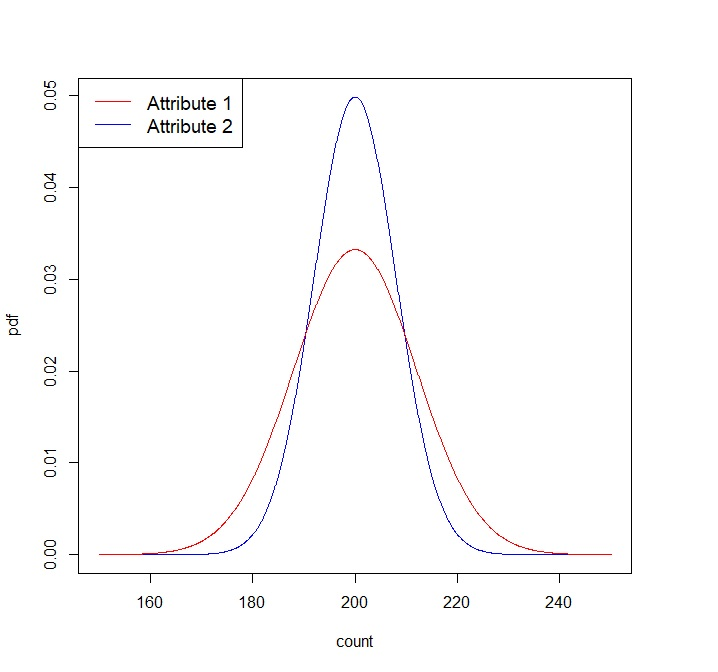
\includegraphics[scale=0.5]{./Images/Distributions.jpg}
	\caption{Distribution of the count of the two attributes} \label{distribution plot}
\end{figure}

In the figure, the mean of the count of the two attributes is 200, and the variances are 64 and 144 respectively. As it can be seen, the height of the probability density function (pdf) for attribute 1 is much lower than that of attribute 2. This means that the count of attribute 1 is less likely to be close to the mean (200 in this case) than attribute 2. Suppose that we see that, in the encrypted database, some encrypted attribute occurs 200 times, our guess would be that this encryption corresponds to attribute 2 in this example. Now we will formalize this attack.

We start by defining statistical distance between two distributions.
\begin{definition}[Statistical distance] \label{statistical distance}
	Let $D_1$ and $D_2$ be two distributions, with pdf $p_1(\cdot)$ and $p_2(\cdot)$ respectively. Statistical distance $d(\cdot,\cdot)$ between $D_1$ and $D_2$ is defined to be:
	\begin{equation}
		d(D_1, D_2) := \int_{-\infty}^{\infty} \lvert p_1(x) - p_2(x) \rvert \  dx.
	\end{equation}
\end{definition}

It is not hard to prove that this definition of statistical distance is a metric. Graphically, this corresponds to the area between the pdf's of the two distributions. It can also be think of as the advantage we have to distinguish two distributions: consider the case where $D_1 = D_2$, then by definition, $d(D_1, D_2) = 0$ so it is impossible for us to differentiate $D_1$ from $D_2$; if $D_1$ and $D_2$ have non-intersecting supports, then $d(D_1, D_2) = 2$, and we can differentiate $D_1$ from $D_2$ with certainty.

In this case, we are interested in two normal distributions with same mean and different variance. We want to derive a lower bound on $d(D_1, D_2)$ given that $D_1 \sim \mathcal{N}(\mu, \sigma^2)$, and $D_2 \sim \mathcal{N}(\mu, \gamma^2\sigma^2)$.

\begin{theorem} \label{thm lb on statistical distance}
	Let $D_1 \sim \mathcal{N}(\mu, \sigma^2)$, and $D_2 \sim \mathcal{N}(\mu, \gamma^2\sigma^2)$ for some $\gamma > 1$. Then
	\begin{equation}
		d(D_1, D_2) \geq 2 \cdot \left( \Phi\left( \gamma\left( \frac{2}{\gamma^2 - 1} \log(\gamma) \right)^{0.5} \right) - \Phi\left( \left( \frac{2}{\gamma^2 - 1} \log(\gamma) \right)^{0.5} \right) \right),
	\end{equation}
	where $\Phi(\cdot)$ is the cdf for standard normal distribution.
\end{theorem}

\textit{Proof:} See appendix \ref{Proof of lb on statistical distance}.

The idea is that, by making $\gamma$ large, we can make $d(D_1,D_2)$ arbitrarily large, so that the advantage generated by the statistical distance is not negligible.

We are ready to present our attack based on \texttt{Padding2}$^{+}$. The idea is to generate the database such that variance of all attributes are equal except one of them - which we want it to be $\gamma^2$ times smaller. Then the encrypted attribute in the database differs the least from the expectation is more likely to be the variable with the smallest variance. But before doing that, we need to show that it is possible to achieve the variances claimed above.

Proof of the claim: Following the standard notation we use in this report, let there be $k$ attributes and $p$ additional insertions, both to be determined later. The idea is to set the distribution of plaintext to $\Pi_0(1) = 1 - k\delta$, and all other $\Pi_0(j)$'s for some $\delta << 1$. We can see immediately if we do so, then $p = k - 1$, if $\delta$ is sufficiently small. Then the variances are:
\begin{align*}
	s^2(1) = & (1 - k\delta) \cdot k \delta + p \cdot \delta (1 - \delta) \\
		   = & (k+p) \delta - (k^2 + p) \delta^2 \\
		   = & (2k - 1) \delta - (k^2 + k - 1) \delta^2 \\
    s^2(j) = & \delta (1 - \delta) + p \frac{1 - \delta}{p} \cdot \left( 1 - \frac{1 - \delta}{p} \right) \\
    	   = & \left(1 - \frac{1}{p}\right) - \left( 1 - \frac{2}{p} \right) \delta - \mathcal{O}(\delta^2) \\
    	   = & \left(1 - \frac{1}{k-1}\right) - \left( 1 - \frac{2}{k-1} \right) \delta - \mathcal{O}(\delta^2) \ \text{for all } j \neq 1
\end{align*}

So the ratio of $s^2(j)$ to $s^2(1)$ for large $k$ is approximately
\begin{align*}
	\frac{1 - \delta}{(2k - 1) \delta - (k^2 + k - 1) \delta^2} 
\end{align*}
which can obviously be made arbitrarily large by picking a large $k$ and $\delta = \mathcal{O}(k^{-2})$. $\square$

\textbf{Attack on Variance} Define he adversary to IND-STAT on \texttt{Padding2}$^{+}$ to be $I = (I_m, I_g)$. Where $I_m$ fixes a $\gamma$ that is large enough, generates plaintext distribution by the process described above with that $\gamma$, and generate $n >> k$ messages sampled from the plaintext distribution. Upon receiving the encrypted database, $I_g$ picks the encrypted attribute $c$ which has its count closest to the mean, and returns his guess as $(m_0,c)$, where $m_0$ is the first attribute with $\Pi_0(1) = 1 - k\delta$.

We can compute the success rate of the attack directly. Let $\xi_1, \cdots, \xi_k$ be random variables corresponds to the counts on the attributes in the encrypted database. So by theorem \ref{thm frequency dist}, we have $\xi_i \sim \mathcal{N}(\frac{n \cdot (p+1)}{k}, n \cdot s^2(i))$. Let $\mu = \frac{n \cdot (p+1)}{k}$, then the probability that attribute 1 is the closest one to the mean can be expressed as:
\begin{align}
  & \prob{\text{attribute 1 is the closest one to the mean}} \\
= & \int_{x} \prob{\text{attribute takes value } x} \cdot \prob{\text{all other attributes takes value further than } x \text{ from } \mu} \ dx \label{VA 1} \\
\approx & \int_{-\infty}^{\infty} p(\xi_1 = x) \cdot \prod_{i = 2}^{k} p(\abs{\xi_i - \mu} > \abs{x - \mu}) \ dx \label{VA 2}\\
= & \int_{-\infty}^{\infty} p(\xi_1 = x) \cdot \prod_{i = 2}^{k} p(\xi_i > \mu + \abs{x - \mu} \text{ or } \xi_i < \mu - \abs{x - \mu}) \ dx \label{VA 3} \\
= & \int_{-\infty}^{\infty} \phi\left(\frac{x - \mu}{\sqrt{n} \cdot s(1)}\right) \cdot \prod_{i = 2}^{k} 2 \cdot \Phi\left(\frac{- \abs{x - \mu}}{\sqrt{n} \cdot s(i)}\right) \label{VA 4}
\end{align}

Equation \ref{VA 1} is just a re-statement of the event. In equation \ref{VA 2}, we have converted the description of the events into their mathematical forms. In the process, we have ignored the contribution of covariance to the likelihood. To go from equation \ref{VA 2} to equation \ref{VA 3}, we turn the event $\abs{\xi_i - \mu} > \abs{x - \mu}$ into expressions with $\xi_i$ on one side and other things on the other, to make it computable. Finally, equation \ref{VA 4} is a direct computation from equation \ref{VA 3}, where $\phi(\cdot)$ and $\Phi(\cdot)$ are the probability density function (pdf) and cumulative density functions respectively.

Unfortunately, it is only possible to compute the integral analytically if $k = 2$. But our goal is to show the existence and correctness of the attack, it is sufficient to use numerical integration to compute this.

\textbf{Numerical Example} As a numerical example, we consider the following input distribution with $k = 6$ and $p = 5$:
\begin{align*}
	\Pi_0(j) = & \begin{cases*}
				   0.95 \quad \text{if } j = 1 \\
				   0.01 \quad \text{otherwise}
		  	     \end{cases*}, \\
	\Pi_i(j) = & \begin{cases*}
				   0.01 \quad \text{if } j = 1 \\
				   0.198 \quad \text{otherwise}
				 \end{cases*} \quad \text{for } i = 1, \cdots,5. 
\end{align*}
The integral in equation \ref{VA 4} in this case evaluates to $0.4054$, which means there is $40.54\%$ chance for the count of attribute 1 in the encrypted database to be the closest one to the mean. This gives an advantage of $0.4054 - \frac{1}{6} = 23.9\%$, which is clearly not negligible. We verify the result by simulating the attack. An advantage of $24.0\%$ is found, with $n = 8000$, and $50,000$ simulation runs of the encryption scheme. $\square$




\textbf{Discussion of the Attack} Note that in equation \ref{VA 4}, the advantage depends on $n$, the number of plaintexts in the database. But our numerical experiments suggest that this dependency is irrelevant. This can be explained intuitively by thinking of the advantage as something generated by the ratio of the variances. In that case, the number of insertions is not a factor.

We argue that the advantage increases as $\gamma$, the ratio between the variances increases. This is verified with a series of experiments similar to the one showed above. The results are summarised in figure \ref{VA advantage table}.

There is also a nice interpretation of the result in terms of statistical distance we have defined in definition \ref{statistical distance}. We expect to differentiate two distributions more easily if they have larger statistical distance. This is indeed the case. Using the estimated statistical distance in theorem \ref{thm lb on statistical distance}, we find a strong correlation between statistical distance and theoretical advantage, as shown in figure \ref{VA advantage table}.

\begin{figure}[H]
	\centering
	\begin{tabular}{cccc}
		$\gamma$ & Advantage (Theoretical est.) & Advantage (Simulation) & Statistical distance \\ \hline
		2.879    & 23.9\%	 & 24.0\% 	& 0.469 \\
		2.073	 & 15.0\%	 & 15.1\%	& 0.338 \\
		1.723    & 10.5\%    & 10.4\%	& 0.257 \\
		1.386    & 5.83\%    & 5.91\%	& 0.157 \\
		1.087    & 1.36\%    & 1.23\%	& 0.040  \\
		1.000    & 0.00\%    & -		& 0.000
	\end{tabular}
	\caption{Relation between $\gamma$ and advantage of Variance attack}
	\label{VA advantage table}
\end{figure}




There are also schemes that are IND-STAT secure but not IND-DIST-CPA secure.
\begin{theorem}
	IND-STAT security does not imply IND-DIST-CPA security.
\end{theorem}

\textit{Proof:} We give an encryption scheme that is IND-STAT secure but not IND-DIST-CPA secure. The construction is similar to \texttt{Padding1}. In addition to the database generated by \texttt{Padding1}, we pad the database further with a dummy attribute, generated by XOR of first two plaintexts in the database. More formally, we define the encryption scheme \texttt{Padding4} = $(Kg, Enc, Dec)$ as:

\begin{figure}[H]
	\begin{center}
		\begin{pchstack}
			\procedure[linenumbering]{$Enc(m_1, \cdots, c_n)$}{%
				\pcfor i \in 1 \cdots n	\\
				\t	D \gets \$(D, \texttt{Padding1.}Enc(m_i)) \\
				\t  D \gets \$(D, Enc_1(m_1 \oplus m_2), Enc_2(False)) \\
				\pcreturn D
			}
		\end{pchstack}
	\end{center}
	\caption{Encryption scheme for \texttt{Padding1}}
\end{figure}
where $\texttt{Padding1.}Enc(\cdot)$ is the encryption function defined for \texttt{Padding1}. And $Kg$ and $Dec$ are the key generation function and decryption functions of \texttt{Padding1} respectively.

\textbf{Part 1: \texttt{Padding4} is IND-STAT secure} \\
We want to show that it is impossible for a statistical attack on the encrypted database generated by \texttt{Padding4}. We rely on the fact that if the attribute columns of the encrypted database is independent of underlying plaintexts, then no statistical information can be inferred. Indeed, the attributes in the encrypted database are in the same order, and have the same number of occurrences regardless of the input plaintexts. Thus, \texttt{Padding4} is IND-STAT secure.

\textbf{Part 2: \texttt{Padding4} is not IND-DIST-CPA secure}
On the other hand, it is easy to attack the database in the IND-DIST-CPA setting. The adversary can generate two raw databases $\{m_1,m_2, \cdots, m_n\}$ and $\{m_1', m_2', \cdots, m_n'\}$ such that $m_1 \oplus m_2 \neq m_1' \oplus m_2'$. After the challenger returns one of the encrypted database, the adversary uses the encryption oracle of $DE$ to encrypt $m_1 \oplus m_2$ and $m_1' \oplus m_2'$. He returns his guess bit $b$ as 0 if the encrypted database contains the encryption of $m_1 \oplus m_2$ and 1 otherwise. The advantage of the adversary is 1. $\square$




\subsection{Security Proofs}
In this section, we will prove that \texttt{Padding1} and \texttt{Padding3} are IND-STAT secure. Security proof for \texttt{Padding1} is almost identical to that of \texttt{Padding4} so we will leave it to the readers. For \texttt{Padding3}, we will use an information-theoretic argument to prove its security.

\begin{theorem}
	\texttt{Padding3} is IND-STAT secure.
\end{theorem}

\textit{Proof:} Recall in theorem \ref{thm frequency dist} we have shown that the distribution of the counts converges to $\mathcal{N}(\frac{n \cdot (p+1)}{k}, n \cdot s^2(j))$ for large $n$. But by construction of \texttt{Padding3}, $s^2(i) = s^2(j) \ \forall i,j$, so we can write the distribution as $\mathcal{N}(\frac{n \cdot (p+1)}{k}, n \cdot s^2)$ for some common variance $s^2$. The covariances between the attributes are equal by construction too. In this form, all parameters of the distribution are available in the public key so the adversary cannot infer anything unknown from the statistics of the database. Therefore, it is impossible to use statistical methods to identify plaintext-ciphertext pairs. $\square$

\textbf{Discussion} The proof above would not work for the trivial encryption scheme. This is because the counts of the encrypted attributes can be modelled by deterministic variables $\xi_1, \cdots, \xi_n$, and these do depend on the count of the input attributes. So by learning these variables, one reveals information about the underlying plaintext.




\subsection{On the Assumption of Absence of Encryption Oracle of $DE$}
Curious readers would realise by this point that IND-STAT is only achievable if the adversary has no access to the encryption oracle of $DE$ - otherwise, he can simply query the encryption oracle with one of the messages he challenged with and return that message with the answer to the query as his output of the game. He wins the game with certainty. But it is not reasonable to make this assumption, given that the underlying encryption scheme is a public-key one. Thus, we have to use something different.

Recall that our database encryption scheme is intended to protect the users from malicious third-party service providers. Since it suffices for the encryption to be deterministic to achieve efficient database queries, we may not want to give the service provider a way to decipher the entries of the database. This can be done easily by making the key `symmetric', i.e. only the users have access to the key and the insertions to the database are done after encryption locally by the users. The same argument can be applied to $PE$ part of the encryption scheme.




\section{Indistinguishability of distribution (IND-DIST)}
In the absence of encryption oracle to $DE$, IND-DIST-CPA is no longer a valid security notion for our application. To adapt to the changes, we define indistinguishability of distribution (IND-DIST) to be the new security notion which is identical to IND-DIST-CPA except that:
\begin{enumerate}
\item The adversary no longer has access to the encryption oracle to $DE$ and $PE$,
\item He can challenge with two completely different message spaces, as long as $p$ and $k$ are fixed.
\end{enumerate}

Let the encryption scheme be $\Sigma = (Kg, \mathcal{E}, \mathcal{D})$. Formally, we define the adversary against $\Sigma$ as tuple $I = (I_d, I_m, I_g)$. $I_d$ takes in the security parameter $1^k$ and generates plaintext sets $M_0, M_1$ and corresponding input distributions (only the actual plaintexts) $\Gamma_0, \Gamma_1$, and the number of inputs $n$. We write the output as $((M_0, \Gamma_0), (M_1, \Gamma_1), n)$. $I_m$ is the message generation algorithm which takes security parameter $1^k$, output of $I_d$, and generate two sequences of inputs to the database $(m_0, m_1)$ (only the actual plaintexts) according to $\Gamma$. The challenger encrypts the inputs $m_b$ using his public key and returns the encrypted database $D$ to the adversary. Finally, $I_g$ is the algorithm which takes input security parameter $1^k$, output of $I_d$ and $I_m$ and encrypted database $D$, and output his guess bit $b'$. He wins if $b = b'$.


\begin{figure}[H]
	\begin{center}
		\procedure{$\text{Exp}_{\text{$\Sigma$, I}}^{\text{IND-DIST}}(1^k)$}{% 
			\pcln b \sample \{0, 1\} \\
			\pcln ((M_0, \Gamma_0), (M_1, \Gamma_1), n) \gets I_d(1^k) \\
			\pcln (\pk, \sk) \gets Kg(1^k, M_b, \Gamma_b) \\
			\pcln (m_0, m_1) \gets I_m(1^k, (M_0, \Gamma_0), (M_1, \Gamma_1), n) \\
			\pcln D \gets \mathcal{E}(1^k, m_b, \pk) \\
			\pcln b' \gets I_g(1^k, (M_0, \Gamma_0), (M_1, \Gamma_1), n, (m_0, m_1), D) \\
			\pcln \pcreturn (b' = b)
		}
	\end{center}
	\caption{IND-DIST adversary}
\end{figure}


The adversary $I$ is legit if:
\begin{enumerate}
\item $n$ is large enough for CLT to hold (we recommend $n \geq 100$),
\item $\abs{M_0} = \abs{M_1}$,
\item Inputs $m$ are truly sampled according to $\Gamma$.
\item All three algorithms runs in polynomial time.
\end{enumerate}
Note that in this setting, the adversary is allowed to generate input distributions $\Gamma_0$ and $\Gamma_1$ such that they are equal.

The advantage of an IND-DIST adversary is defined as
\begin{equation}
\text{Adv}_{\text{$\Sigma$, I}}^{\text{IND-DIST}}(1^k) = \prob{\text{Exp}_{\text{$\Sigma$, I}}^{\text{IND-DIST}}(1^k) \Rightarrow \text{true}} - \prob{\text{Exp}_{\text{$\Sigma$, I}}^{\text{IND-DIST}}(1^k) \Rightarrow \text{false}}.
\end{equation}

With a standard probability argument, we can show that
\begin{equation}
\text{Adv}_{\text{$\Sigma$, I}}^{\text{IND-DIST}}(1^k) = 2\prob{\text{Exp}_{\text{$\Sigma$, I}}^{\text{IND-DIST}}(1^k) \Rightarrow \text{true}} - 1.
\end{equation}

We say that scheme $\Sigma$ is secure under IND-DIST if $\text{Adv}_{\Sigma, \text{I}}^{\text{IND-DIST}}(1^k)$ is negligible in $k$.


\textbf{A Useful Fact:} Define the maximum key probability $\text{mkp}_\Sigma(1^k)$ for encryption scheme $\Sigma = (Kg, \mathcal{E}, \mathcal{D})$ with security parameter $1^k$ as:
\begin{equation}
	\text{mkp}_\Sigma(1^k) = \max_{v} \prob{\pk = v \mid (\pk, \sk) \gets Kg(1^k)} + \max_{w} \prob{\sk = w \mid (\pk, \sk) \gets Kg(1^k)}
\end{equation}

We claim that if $\Sigma$ is IND-CPA secure, then $\text{mkp}_\Sigma(1^k)$ is negligible in $k$. 

\textit{Proof:} The proof can be seen as a generalization to proposition 4.1 in \cite{Bellare2007}. We suppose for the sake of contrary that $\text{mkp}_\Sigma(1^k)$ is not negligible, and we demonstrate that we can construct an IND-CPA adversary against $\Sigma$. By construction, if $\text{mkp}_\Sigma(1^k)$ is not negligible then either $\max_{v} \prob{\pk = v \mid (\pk, \sk) \gets Kg(1^k)}$ is not negligible or $\max_{w} \prob{\sk = w \mid (\pk, \sk) \gets Kg(1^k)}$ is not.

In the first case, it means that certain public key is generated with significant probability. We can simply run the key generation algorithm repetitively until the public key part of the key is that key. If $\max_{v} \prob{\pk = v \mid (\pk, \sk) \gets Kg(1^k)} = p$, then we only need $\mathcal{O}(1/p)$ runs of the key generation algorithm to find out the key pair. After that, we can freely decrypt any message we want, so we break $\Sigma$ with certainty.

Similarly, if $\max_{w} \prob{\sk = w \mid (\pk, \sk) \gets Kg(1^k)} = p$ is not negligible, we can run the key generation algorithm $\mathcal{O}(1/p)$ times to find the corresponding secret key, and decrypt any message we want afterwards. $\square$


\begin{theorem} \label{thm IND-STAT 1}
Let $I = (I_d, I_m, I_g)$ be the IND-STAT adversary against \texttt{Padding1}, then:
\begin{equation}
	\text{Adv}_{\text{\texttt{Padding1}, I}}^{\text{IND-DIST}}(1^k) \leq \text{mpk}_{DE}(1^k) + \text{mpk}_{PE}(1^k)
\end{equation}	
\end{theorem}

\textit{Proof:} Without encryption oracles, the adversary can only win the security game by guessing the public and secret keys of $DE$ and $PE$. There are three cases to consider:

\textbf{Case 1: $M_0 = M_1$, attributes have the same frequencies} \\
In this case, encryption of the two databases are identical, it is impossible to tell them apart in any way. Thus, $\text{Adv}_{\text{\texttt{Padding1}, I}}^{\text{IND-DIST}}(1^k) = 0$.

\textbf{Case 2: $M_0 = M_1$, attributes have different frequencies} \\
The adversary has to decipher the auxiliary column to retrieve the counts on the attributes. He succeeds with probability at most $\text{mpk}_{PE}(1^k)$.

\textbf{Case 3: $M_0 \neq M_1$} \\
If $M_0 \neq M_1$, then the encryptions will have different ciphertexts. The adversary wins the security game by encrypting (or equivalently decrypting) the attributes in $M_0$ and $M_1$ and check if the ciphertext comes from the first or the second set. He makes the right guess of the public key or the secret key with probability bounded by $\text{mpk}_{DE}(1^k)$.

The overall advantage of the adversary is bounded by the sum of the advantages. Whence we get
\begin{equation*}
\text{Adv}_{\text{\texttt{Padding1}, I}}^{\text{IND-DIST}}(1^k) \leq \text{mpk}_{DE}(1^k) + \text{mpk}_{PE}(1^k). \square
\end{equation*}


\begin{theorem}
	Let $I = (I_d, I_m, I_g)$ be the IND-STAT adversary against \texttt{Padding3}, then:
	\begin{equation}
	\text{Adv}_{\text{\texttt{Padding3}, I}}^{\text{IND-DIST}}(1^k) \leq \text{mpk}_{DE}(1^k) + \text{mpk}_{PE}(1^k)
	\end{equation}	
\end{theorem}

\textit{Proof:} Let $\xi_1, \cdots, \xi_k$ be the counts of the attributes in the encrypted database. By construction $\xi_i$ have the same distribution so they are indistinguishable from each other from a statistical point of view. It also means that
\begin{equation*}
	\prob{(\xi_1, \cdots, \xi_k) \mid \Gamma} = \prob{(\xi_1, \cdots, \xi_k)},
\end{equation*}
i.e. the joint distribution is independent of the input distribution $\Gamma$. This implies
\begin{equation*}
	\prob{(\xi_1, \cdots, \xi_k) \mid \Gamma_0} = \prob{(\xi_1, \cdots, \xi_k) \mid \Gamma_1}
\end{equation*}
so the advantage of the adversary generated through the counts is 0. The proof reduces to theorem \ref{thm IND-STAT 1}. Thus the claimed advantage. $\square$













\chapter{Conclusion}
In this chapter, we will summarize the main results and conclude our studies.


\section{Summary of Results}
In the studies, we have seen that the current implementations of EDB based on property-preserving encryption schemes are not practical secure even though the underlying schemes have security guarantees under their security notions. This happens because either the assumptions of the security notion are not met, or the security notion itself is not strong enough to protect EDB from practical attacks (such as frequency attack).

We have constructed alternative schemes as an attempt to defeat statistical attacks on the database. The schemes are based on padding, so as to hide any statistical information in the EDB. \texttt{Padding1} is the full padding scheme which hides all statistical information. However, it is not space efficient hence not a practical scheme. We modified the scheme to pad probabilistically, giving us \texttt{Padding2} and \texttt{Padding3}.

To analyse the security of the new schemes, we proposed new security notion IND-DIST-CPA (reduced to IND-DIST later), and IND-STAT and proven some key results:
\begin{enumerate}
\item \texttt{Padding1} and \texttt{Padding3} are IND-DIST-CPA and IND-DIST secure,
\item IND-DIST-CPA and IND-STAT are not comparable notions, and
\item \texttt{Padding1} and \texttt{Padding3} are IND-STAT secure.
\end{enumerate}

In the process to show IND-DIST-CPA and IND-STAT are not comparable, we proposed a new type of statistical attack known as variance attack. This attack can differentiate variables with the same mean and different variance with provable success rate.




\section{Practical Concerns with Proposed Encryption Schemes}
The number of dummy insertions for all the proposed schemes are related to the number of attributes in the database. In practice, this can be a huge number. As a numerical example, suppose that the database has 10 columns, and each column has 4 possible values to take. That means there are $4^{10} = 2^{20}$ attributes in total. This is simply impractical for \texttt{Padding1}. For \texttt{Padding3}, optimization problem 2 in section \ref{OP2} may be impossible to solve in reasonable amount of time.

To tackle with this problem, we propose to use \texttt{Padding3} on groups of columns for which the user really want to hide correlation. For instance, in medical records, we want to encrypt diagnosis of disease and treatment together (a pair corresponds to an attribute) but we may not care about the correlation between admission date and gender so they can be encrypted separately.

It is also advised to encrypt columns with small attribute space using conventional probabilistic encryption scheme. This is because the security guarantee of our padding based schemes do depend on the number of attributes in the columns.




\section{Further Work}
So far our scheme aims to protect the users from faithful but curious service provider in terms of storage. But in practice, the adversary has other means to attack the database. For instance, our construction requires shuffling of rows in the database. A dishonest service provider does not necessarily follow the rules. If he knows the underlying plaintext, and a few groups of the insertions, he can just take intersection of those groups to find out the common ciphertext - which will certainly be the encryption to the plaintext above.

There are many more leakage based attacks possible. \cite{cryptoeprint:2016:718} provides an excellent account on them. For instance, the adversary may use queries to recover the underlying plaintexts via frequency attack similar to \cite{Naveed:2015:IAP:2810103.2813651}. \cite{Islam12accesspattern, Liu:2014:SPL:2580107.2580271} have proposed query schemes to protect the users from the later attack. But they are not successful in hiding user queries once the access pattern is leaked.

In the future, we wish to give new security notions to incorporate user queries and other mechanisms which may leak information. We want to develop new schemes which can achieve provable security under the new notions.











\bibliographystyle{plain}
\bibliography{Reference}{}

\appendix
\chapter{Proof of theorem \ref{thm frequency dist}} \label{proof of thm frequency dist}
\textit{Proof:} To prove the theorem, we need to use Central Limit Theorem. The variant used in the proof is perceived by Russian mathematician Aleksandr Lyapunov where the random variables only need to be independent, not necessarily identical.


\begin{theorem}[Central Limit Theorem (Lyapunov)] \label{CLT}
Let $\{X_1, \cdots, X_n\}$ be a sequence of $n$ independent distributed random variables with $E(X_i) = \mu_i$ and $Var(X_i) = \sigma_i^2$. Define $s_n^2 = \sum_{i = 1}^{n} \sigma_i^2$. If for some $\delta > 0$, Lyapunov's condition \\
\begin{align*}
	\lim_{n \rightarrow \infty} \frac{1}{s_{n}^{2+\delta}} \sum_{i=1}^{n} E\left[\:\abs{X_i - \mu_i}^{2+\delta}\right] = 0
\end{align*}
is satisfied, then as $n$ approaches infinity,
\begin{align*}
	\frac{1}{s_n} \sum_{i=1}^{n} (X_i - \mu_i) \xrightarrow[]{d} \mathcal{N}(0, 1).
\end{align*}
\end{theorem}


Our proof will take three steps. In the first step, we will compute $s_{n(p+1)}^2(j)$. After that, we will argue that the Lyapunov's condition is indeed satisfied. Finally, we will apply CLT and derive equation \ref{frequency dist}.

\textbf{Step 1:} We compute $s_{n(p+1)}^2(j)$ defined in the theorem as:
\begin{align}
	s_{n(p+1)}^2(j) & = \sum_{i=1}^{n(p+1)} Var(X_i^j) \label{thm1 1.1} \\
		 		 	& = \sum_{i=1}^{n(p+1)} \Pi_{index(i)}(j) \cdot (1 - \Pi_{index(i)}(j)) \label{thm1 1.2} \\
		  		 	& = \sum_{l = 1}^{n} \sum_{i = 0}^{p} \Pi_i(j) (1 - \Pi_i(j))  \label{thm1 1.3}\\
		  		 	& = n \cdot \sum_{i = 0}^{p} \Pi_i(j) (1 - \Pi_i(j)) \label{thm1 1.4}.
\end{align}


The computation is straightforward. In equation \ref{thm1 1.1}, we use the definition of $s_{n(p+1)}^2(j)$ in theorem \ref{CLT}. For Bernoulli distribution with success probability $p$, the variance is $p \cdot (1 - p)$, hence equation \ref{thm1 1.2}. But by construction, we sample from $\Pi_i(j)$ for $i \in \{0, \cdots, p\}$ $n$ times each (In this case, we treat the actual input as a random variable too.), so we can re-write the equation as \ref{thm1 1.3}. Finally, the inner summation is not dependent on $l$, so the double summation is nothing but $n$ times of the inner summation in \ref{thm1 1.4}.


\textbf{Step 2:} As $X_i^j$'s are Bernoulli random variables, all moments exist, whence Lyapunovs condition is satisfied for any $\delta > 0$. So we can apply CLT to conclude that as n goes to infinity,
\begin{align}
	\frac{1}{s_{n(p+1)}(j)} \sum_{i=1}^{n(p+1)} (X_i^j - \mu_i) \xrightarrow[]{d} \mathcal{N}(0, 1). \label{thm1 2.1}
\end{align}


\textbf{Step 3:} In reality, the observed variable is $\sum_{i} X_i^j$, or plainly, the number of occurrences of attribute $j$. We can obtain the distribution of $\sum_{i} X_i^j$ from equation \ref{thm1 2.1} as:
\begin{align*}
	\sum_{i=1}^{n(p+1)} (X_i^j - \mu_i) & \xrightarrow[]{d} \mathcal{N}\left(0, s_{n(p+1)}^2(j)\right) \\
	\sum_{i=1}^{n(p+1)} X_i^j - \sum_{i=1}^{n(p+1)} \mu_i & \xrightarrow[]{d} \mathcal{N}\left(0, s_{n(p+1)}^2(j)\right) \\
	\sum_{i=1}^{n(p+1)} X_i^j - \sum_{l = 1}^{n} \sum_{i=0}^{p} \mu_i & \xrightarrow[]{d} \mathcal{N}\left(0, s_{n(p+1)}^2(j)\right) \\
	\sum_{i=1}^{n(p+1)} X_i^j - \sum_{l = 1}^{n} \sum_{i=0}^{p} \Pi_i(j) & \xrightarrow[]{d} \mathcal{N}\left(0, s_{n(p+1)}^2(j)\right) \\
	\sum_{i=1}^{n(p+1)} X_i^j - n \cdot \frac{p+1}{k} & \xrightarrow[]{d} \mathcal{N}\left(0, s_{n(p+1)}^2(j)\right) \\
	\sum_{i=1}^{n(p+1)} X_i^j & \xrightarrow[]{d} \mathcal{N}\left(\frac{n \cdot (p+1)}{k}, s_{n(p+1)}^2(j)\right) \numberthis \label{thm1 3.1} \qquad \square
\end{align*}
\chapter{Justification of the claim in \ref{thm5}} \label{Justification of claim P2 1}
\textbf{Claim}: Statistical distance between two databases generated by \texttt{Padding2}$^{+}$ can be made arbitrarily small.

To justify the claim, recall that the probability density function of multivariate normal distribution (in the non-degenerate case) takes the form:
\begin{align*}
	f(\xi_1, \cdots, \xi_k) = \frac{\exp \left( - \frac{1}{2} (\xi - \mu)^{\text{T}} \Sigma^{-1} (\xi - \mu) \right)}{\sqrt{\bigl\lvert 2\pi\Sigma \bigr\rvert}},
\end{align*}
where mean is $\mu$ and variance is $\Sigma$. Suppose we have another multivariate normal distribution with mean $\mu^{*}$ and variance $\Sigma^{*}$, we can make a crude bound the difference of the two probability density functions by:
\begin{align*}
  & \text{differnce of pdf} \\
= & \bigl\lvert \frac{\exp \left( - \frac{1}{2} (\xi - \mu)^{\text{T}} \Sigma^{-1} (\xi - \mu) \right)}{\sqrt{\bigl\lvert 2\pi\Sigma \bigr\rvert}}
- \frac{\exp \left( - \frac{1}{2} (\xi - \mu^{*})^{\text{T}} (\Sigma^{*})^{-1} (\xi - \mu^{*}) \right)}{\sqrt{\bigl\lvert 2\pi\Sigma^{*} \bigr\rvert}} \bigr\rvert \\
\leq & \bigl\lvert \frac{\exp \left( - \frac{1}{2} (\xi - \mu)^{\text{T}} \Sigma^{-1} (\xi - \mu) \right)}{\sqrt{\bigl\lvert 2\pi\Sigma \bigr\lvert}} \bigr\rvert
+ \bigl\lvert \frac{\exp \left( - \frac{1}{2} (\xi - \mu^{*})^{\text{T}} (\Sigma^{*})^{-1} (\xi - \mu^{*}) \right)}{\sqrt{\bigl\lvert 2\pi\Sigma^{*} \bigr\rvert}} \bigr\rvert \\
\leq & \frac{1}{\sqrt{\lvert2\pi\Sigma\rvert}} + \frac{1}{\sqrt{\lvert 2\pi\Sigma^{*} \rvert}} \\
= & \frac{1}{(2\pi)^k} \left( \frac{1}{\lvert \Sigma \rvert} + \frac{1}{\lvert \Sigma^{*} \rvert} \right).
\end{align*}
But $\lvert \Sigma \rvert$ is bounded from below by $k \cdot v$, where $v$ is the smallest eigenvalue of $\Sigma$. Similarity, we can bound $\lvert \Sigma^{*} \rvert$ by $k \cdot v^{*}$, where $v^{*}$ is the smallest eigenvalue of $\Sigma^{*}$. So the difference of pdf is bounded by
\begin{align*}
	\frac{k(v + v^{*})}{(2\pi)^k}.
\end{align*}
By picking the covariance matrix carefully, the final expression can be made negligible in the security parameter. So there is no realization of the encryption scheme for which the adversary can differentiate the two databases.
\chapter{Proof of Theorem \ref{thm lb on statistical distance}} \label{Proof of lb on statistical distance}

\textit{Proof:} The lower bound comes from the centre part of the integral. The proof is nothing more than direct computation. First of all, we wish to find the intersection points of the two pdf's. This is done by setting the two pdf's equal, and solve for $x$:
\begin{align*}
\frac{1}{\sqrt{2\pi \sigma^2}} \exp \left\{ -\frac{(x - \mu)^2}{2\sigma^2} \right\} & = \frac{1}{\sqrt{2\pi \gamma^2 \sigma^2}} \exp \left\{ -\frac{(x - \mu)^2}{2 \gamma^2\sigma^2}\right\} \\
\gamma & = \exp  \left\{ \frac{(x - \mu)^2}{2\sigma^2} - \frac{(x - \mu)^2}{2 \gamma^2\sigma^2} \right\} \\
\log(\gamma) & = \frac{(x - \mu)^2}{2\sigma^2} - \frac{(x - \mu)^2}{2 \gamma^2\sigma^2} \\
2 \gamma^2\sigma^2 \log(\gamma) & = (\gamma^2 - 1) (x - \mu)^2 \\
x &= \mu \pm \left( \frac{2 \gamma^2\sigma^2}{\gamma^2 - 1} \log(\gamma) \right)^{0.5} \\
x &= \mu \pm \gamma \sigma \left( \frac{2}{\gamma^2 - 1} \log(\gamma) \right)^{0.5} \numberthis \label{pdf intersections}
\end{align*}

Then it is immediate that:
\begin{align*}
d(D_1, D_2) = & \int_{-\infty}^{\infty} \lvert p_1(x) - p_2(x) \rvert \  dx \\
\geq & \int_{\mu - \left( \frac{2 \gamma^2\sigma^2}{\gamma^2 - 1} \log(\gamma) \right)^{0.5}}^{\mu + \left( \frac{2 \gamma^2\sigma^2}{\gamma^2 - 1} \log(\gamma) \right)^{0.5}} \lvert p_1(x) - p_2(x) \rvert \  dx \\
=   & \int_{\mu - \left( \frac{2 \gamma^2\sigma^2}{\gamma^2 - 1} \log(\gamma) \right)^{0.5}}^{\mu + \left( \frac{2 \gamma^2\sigma^2}{\gamma^2 - 1} \log(\gamma) \right)^{0.5}}  p_2(x) - p_1(x) \  dx \\
=   & 2 \cdot \left( \Phi\left( \gamma\left( \frac{2}{\gamma^2 - 1} \log(\gamma) \right)^{0.5} \right) - \Phi\left( \left( \frac{2}{\gamma^2 - 1} \log(\gamma) \right)^{0.5} \right) \right). \square
\end{align*}


\end{document}

